%: ----------------------- introduction file header -----------------------
% the code below specifies where the figures are stored
\graphicspath{{5/figures/}}

\chapter{Automatic Chord Estimation}
\label{chp:chord_estimation}

% Context / Purpose
The previous chapter was able to reformulate timbre similarity as a well-defined task that used objective information for development and evaluation.
Automatic chord estimation, one of the oldest subtopics in the field of content-based MIR, embodies nearly the polar opposite scenario, being rather ill-defined and depending on subjective information almost exclusively.
As such, it provides an interesting case study with which to test the limits of deep learning.
% Goal
In addition to the standard objective of looking to advance the state of the art in a chosen application domain, this chapter seeks to explore the limitations of deep learning as applied to complex music intelligence task.
A thorough investigation serves to not only offer insight into the application of deep learning methods to future problems in content-based MIR, but also culminate in a better understanding of the chord estimation task itself.


\section{Context}
\label{sec:context}

In this section, the prerequisite knowledge necessary to appreciate a thorough treatment of automatic chord estimation systems is addressed.
% Concepts - Build an understanding of musical harmony
First, a basic review of Western tonal theory sets out to define key music concepts, and thus provides a language with which to discuss the problem.
% Practical considerations - Chord syntax
This is followed by a brief outline of the syntax used here to compactly notate chords.
% Motivation -- why
The problem domain is then jointly motivated by potential use-cases and the observed needs of online music communities.
% Limitations -- caveats
Finally, known limitations are detailed to contextualize both assumptions and any conclusions drawn from this work.



\subsection{Musical Foundations}
\label{subsec:musical_foundations}

% Acoustics and perceptions -- pitch, tones, octaves, frequency
% -------------------------
To understand the chord estimation task is to understand the concepts on which it is built.
% To get to the top, start at the bottom.
The most atomic unit in the acoustic realm of chords is a \emph{tone}, defined here as a pitched sound object.
Pitch is defined as the perceptual phenomena whereby a sound stimulus can be matched to the frequency of a pure sinusoid, known as the fundamental frequency.
As a result, sounds can be naturally ordered by fundamental frequency on a scale from low to high.
An \emph{octave} is defined as the doubling of a quantity, and exhibits a special relationship in human perception by which two tones, differeing in fundamental frequency by an integer power of 2, are perceived as being similar; this phenomena is referred to as octave equivalence \cite{?}.
% Pitch helix here?

% Notes and tuning systems
% ------------------------
A \emph{note} is the musical counterpart of a tone, and the two are related by way of a tuning system.
While there are a multiplicity of tuning systems, this work will exclusively consider 12-Tone Equal Temperament, or 12-TET, named for the 12 discrete, equally spaced tones between within an octave.
The relationship between notes and tones in 12-TET is defined by the following:

\begin{equation}
\label{eq:tuning}
f_{pitch} = f_{tuning} * 2 \exp(\frac{n_{index} - 48}{N})
\end{equation}

\noindent where $N$ is the number of notes per octave, $n_{index}$ is an integer note index, $f_{tuning}$ is the reference frequency, in Hertz, on which , and $f_{pitch}$ is the fundamental frequency, in Hertz, of the corresponding tone.
In 12-TET, the \emph{unique pitch classes} within an octave are named, given by the ordered set, $\mathcal{P}$:

\begin{equation}
\label{eq:pitch_classes}
\mathcal{P} = \{C, C\sharp / D\flat, D, D\sharp / E\flat, E, F, F\sharp / G\flat, G, G\sharp / A\flat, A, A\sharp / B\flat, B\}
\end{equation}

Here, sharps, $\sharp$, and flats, $\flat$, are symbols used to indicate the raising or lowering of a note by one semitone, respectively.
Note that due to this particular tuning system, some pitch classes can be spelled with either a sharp or a flat, e.g. $A\sharp = B\flat$, a property known as \emph{enharmonic equivalence}.
An absolute note name, consisting of a pitch class, $p$, and an octave, $o$, is given by the following as a function of absolute note index, such that $n_{index}=0~\to~C0$, $n_{index}=12~\to~C1$, etc.:

\begin{align*}
p = \mathcal{P}[mod(n_{index}, 12)] \\
o = \lfloor~n_{index} / 12~\rfloor
\end{align*}

In contemporary music, standard concert tuning equates $A4=440Hz$; classically, the tuning frequency is defined such that it falls in the performance range of a majority of instruments to be matched exactly, and hence the offset in Eq. \ref{eq:tuning}.
% dunno I like / want this sentence
Were the tuning system and reference frequency universally constant, the concepts of tones and notes would be equivalent; it should be noted, however, this is not the case.

% Intervals
% ---------
Most\footnote{But not all, as in the case of John Cage's \emph{4'33''}, which contains none.} real music combines many different notes, and thus it is useful to define an \emph{interval} is defined as the relative semitone distance between two notes.
Whereas notes are atomic, intervals are the bonds in a harmonic molecule.
The interval between consecutive pitch classes is referred to as a \emph{semitone}, with a step size of 1, and a step size of 2 is known as a \emph{whole tone}.
Intervals are critical to music perception because they are generally perceived as similar regardless of pitch height, e.g. the interval from C4 to G4 sounds the same as the interval from F4 to C5, both being seven semitones.

% Scales, chords, and keys; a circular quagmire
% ------------------------
From here, three interdependent harmonic concepts are built through the simultaneous and sequential combination of notes and, as a result, intervals: scales, chords, and keys.
It is crucial to recognize that each is an emergent quality of the same fundamental parts, and efforts to define one in terms of another results in circular logic.
For clarity, the relationships between the various entities discussed so far are diagrammed hierarchically in Figure \ref{fig:concept_hierarchy}.

That said, an ordered set of intervals in known as a scale, of which the \emph{diatonic} is the most widely used in common practice music.
It consists of eight semitone scale degrees, and thus seven intervals, given by the following:

\begin{align*}
\{2, 2, 1, 2, 2, 2, 1\}
\end{align*}

Rotating this sequence circularly results in different \emph{modes}, of which two are common in contemporary popular music: \emph{major}, with a rotation of 0; and \emph{minor}, with a rotation to the right of 3.
Starting from 0, the semitone values of these scales are expressed by the following:

\begin{align*}
\texttt{maj} = \{0, 2, 4, 5, 7, 9, 11, 12\} \\
\texttt{min} = \{0, 2, 3, 5, 7, 8, 10, 12\} \\
\end{align*}

These sequences can be used to recover a scale by circularly indexing the set of pitch classes given in \ref{eq:pitch_classes}.
The starting pitch classon which the scale is based is referred to the \emph{tonic}, and lends its name to the scale.
To illustrate, a C Major and A minor scale are given as follows:

\begin{align*}
\mathcal{C}_{major} = \{C, D, E, F, G, A, B\} \\
\mathcal{A}_{minor} = \{A, B, C, D, E, F, G\} \\
\end{align*}

One should observe that these two scales, with different modes and tonics, are composed of identical notes.
These scales are known as each other's relative major and minor, respectively, and share a strong perceptual affinity.


% \begin{table}[h]
% \begin{center}
% \caption{Degrees, names, semitones, and intervals of the Major (Ionian) scale.}
% \label{tab:diatonic}
% \begin{tabular}{c | c | c | c }
% Degree & Name & Semitones & Interval \\
% \hline
% 1st & Tonic & 0 & -- \\
% 2nd & Supertonic & 2 & +2 \\
% 3rd & Mediant & 4 & +2 \\
% 4th & Subdominant & 5 & +1 \\
% 5th & Dominant & 7 & +2 \\
% 6th & Submediant & 9 & +2 \\
% 7th & Leading Tone & 11 & +2\\
% 8th & Tonic (Octave) & 12 & +1 \\
% \hline
% \end{tabular}
% \end{center}

% Chords, by the book
% -------------------
Proceeding from scales, a \emph{chord} is classically conceived as a simultaneous grouping of notes.
One of the most important chord types in Western tonal theory is the \emph{triad}, on which many other theoretical constructs are built.
Comprised of three notes, a triad is built by taking the second and fourth scale degrees from a chosen starting point, referred to as the root.
For example, this expansion is given for the C-major scale in Table \ref{tab:major_triads}.

\begin{table}[h!]
\begin{center}
\caption{Roman numeral, quality, semitones, and intervals of triads in the Major scale.}
\label{tab:major_triads}
\begin{tabular}{c | c | c | c }
Roman Numeral & Quality & Semitones & Intervals \\
\hline
I & Major & \{0, 4, 7\} & \{+4, +3\}\\
ii & minor & \{2, 5, 9\} & \{+3, +4\}\\
iii & minor & \{4, 7, 7\} & \{+3, +4\}\\
IV & Major & \{5, 9, 12\} & \{+4, +3\}\\
V & Major & \{7, 11, 2\} & \{+4, +3\}\\
vi & minor & \{9, 0, 4\} & \{+3, +4\}\\
vii$^\circ$ & diminished & \{11, 2, 5\} & \{+3, +3\}\\
I & Major & \{0, 4, 7\} & \{+4, +3\}\\
\hline
\end{tabular}
\end{center}
\end{table}

For a given chord, the \emph{root} is defined as the home note on which the intervals are stacked, and the \emph{quality} determined by the relationship of the intervals to the root.
An interval of 4 semitones is known as a \emph{major third} and 3 semitones a \emph{minor third}, sharing a commonality with the third scale degree of the major and minor scales, respectively.
Therefore, the qualities of the first six chords in the table are named for their relationship with the corresponding major and minor scales; the vii$^\circ$ chord, however, is named differently because it contains two minor thirds.

% Key
% ---
Sharing much common ground with scales and chords, a \emph{key} identifies a point of harmonic stability in reference to a tonic and its corresponding triad.
Accordingly, the keys conventionally take one of the pitch classes and either a major or minor quality, e.g. $E-major$ or $C\sharp-minor$.
Key is integral to the discussion here, because its impression or expectation establishes a harmonic framework with which to parse musical information, leading to the understanding of notes and intervals as they relate to scales and chords.


% Attempts to define a chord
While much of this theory can be detailed specifically, real music is by no means so well behaved.
As a result, the practical definition of a ``chord'' is open to some interpretation, and may take multiple meanings.
For example, \cite{McVicar2013} collects three possible definitions, restated here:

\begin{enumerate}
\item \emph{Everyone agrees that \emph{chord} is used for a group of musical tones.}
\item \emph{Two or more notes sounding simultaneously are known as a chord.}
\item \emph{Three or more pitches sounded simultaneously or functioning as if sounded simultaneously.}
\end{enumerate}

% Pitch and notes
Additionally, \cite{Harte2010} expands the scope of (2) in order to describe all tonal music, ``allow[ing] a chord to comprise zero or more notes.''
The various flavors of defintions begs an obvious question: what makes the concept of a chord so hard to pin down?

% Chord composition
Much of this difficulty stems from the fact that the relative importance of the individual notes in a collection may change in different contexts.
In practice, a chord is named based on three subjective criteria: its root, its contributing intervals, and how these two relate to the key.
Therefore, as will be shown shortly, a chord can easily take a different name if any of these decisions are changed or reweighted.
% A ``root'' is the note in a chord that serves as a point of \emph{internal} harmonic stability; conversely, a ``key'' is itself a chord which serves as a point of \emph{external} harmonic stability.

% Why is it so hard to define a chord? Let's look at some examples
Having briefly reviewed Western tonal theory, a deeper understanding of the variation inherent to defining a chord can be obtained by exploring a few simple examples.
The one invariant property shared by all defintions named previously is the idea that a pitch collection may be understood as a single harmonic object.
The time span over which this phenomena may unfold, however, is flexible.
To illustrate the point, consider the three bars notated in Figure \ref{fig:expanded_major}, where a major chord is written as a true simultaneity, an arpeggiation, and as an series of non-overlapping quarter notes, respectively.
In this instance, the degree of overlap in time is expanded until it no longer exists, and yet the collection of notes continues to function as a coherent harmonic object.

\begin{figure}[t]
\centering
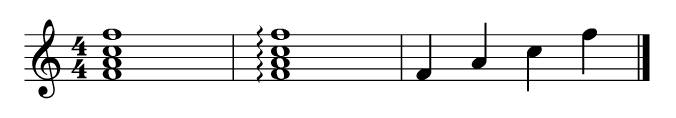
\includegraphics[width=\textwidth]{expanded_major}
\caption{writeme}
\label{fig:expanded_major}
\end{figure}

On the other hand, as shown in Figure \ref{fig:nonchord_tones}, the simultaneous sounding of different notes does not necessarily give rise to the perception of different chords.
Here, a major triad is sustained under the first several degrees of its scale.
While three notes in the upper voice are contained in the C-major triad, the others --the D, F, and A-- are referred to as ``nonchord'' tones.
These extra notes are explained away in the overall harmonic scene, as they fall on metrically weak beats, are comparatively short in duration, and quickly move to notes that \emph{are} in the chord.
These embellishments do not contribute to the harmonic center of the phrase, and the bar can still be understood as a stable C-major chord.

\begin{figure}[t]
\centering
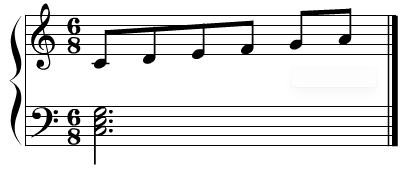
\includegraphics[width=\textwidth]{nonchord_tones}
\caption{writeme}
\label{fig:nonchord_tones}
\end{figure}

A last example, shown in Figure \ref{fig:mthomework}, demonstrates the level of complexity and inherent subjectivity that may arise in the process of describing real music with chords.
Referred to as \emph{harmonic analysis}, this exercise is performed in an effort to understand the harmonic content in a theoretical manner.
Here, an excerpt of a score has been analyzed, with chords notated under the original parts.
Even in this instance, where the individual is able to operate directly on the symbolic representation, it is common to find alternate interpretations of the same musical content.
Conversely, annotations resulting from sound recordings, as opposed to a score, are referred to as \emph{chord transcriptions}.
Often the recording itself is the only musical artifact to consider, introducing even more room for subjectivity.

\begin{figure}[t]
\centering
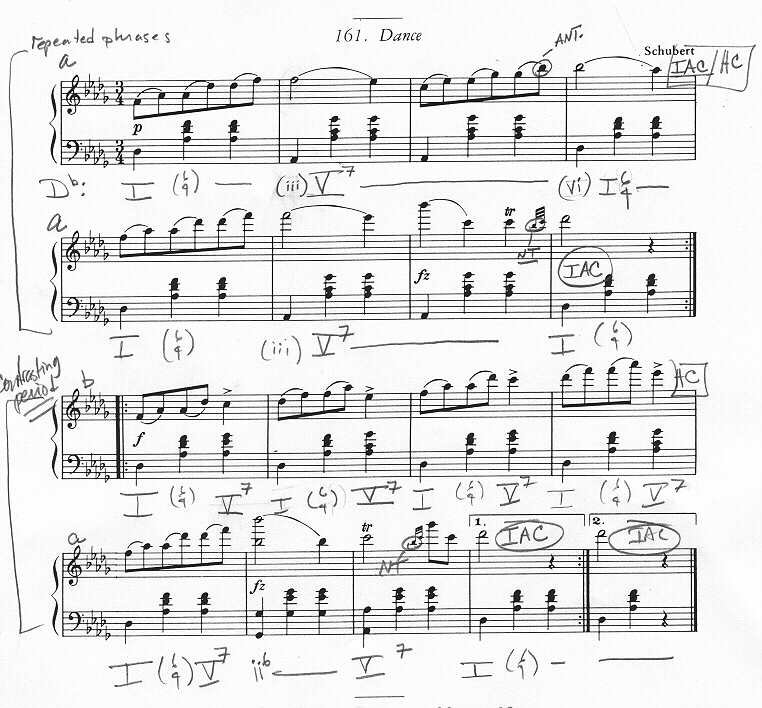
\includegraphics[width=\textwidth]{practicekey2.jpg}
\caption{A sample harmonic analysis, performed as a music theory exercise.}
\label{fig:mthomework}
\end{figure}


% Skilled musicans are quite robust in the ability to assign chord labels to musical scenes despite an occasionally opaque decision making process, and it is an exciting challenge to produce a computational system with a similar capacity.


\subsection{Chord Syntax}
\label{sec:chord_syntax}

It is a pragmatic, but ultimately necessary, preliminary step to define a standard syntax for compactly notating chords.
Much of the pioneering work in this space was performed by Harte \cite{Harte2010}, and many of these conventions are utilized here.
Going forward, chords expressed in this scheme are stylized with a fixed-width font, e.g. \texttt{A:min}.

Firstly, Harte's general chord notation is described by the following four-part symbolic description:

\begin{equation}
\{r\}:\{q\}(i)/\{b\}
\end{equation}

\noindent Every chord name begins with a root $r$ in the form of a pitch class, optionally modified by zero or more sharps or flats, or one of two reserved characters: \texttt{N} for the ``null'' no-chord condition, or \texttt{X} for the special case in which the musical content cannot be described harmonically.

The root is potentially followed by a quality shorthand, $q$, separated by a colon and implying a particular set of note intervals.
Though there are a large number of possible chord qualities, this is often limited to a particular subset in practice.
Those considered in this work are indicated in the following table:

\begin{table}[t]
\begin{center}
\caption{Chord quality names and corresponding relative semitones.}
\label{tab:qualities}
\begin{tabular}{l | c | c}
Name & Shorthand & Semitones \\
\hline
Major & \texttt{maj} & $\{0, 4, 7\}$ \\
Minor & \texttt{min} & $\{0, 3, 7\}$ \\
Major 7 & \texttt{maj7} & $\{0, 4, 7, 11\}$ \\
Minor 7 & \texttt{min7} & $\{0, 3, 7, 10\}$ \\
Dominant 7 & \texttt{7} & $\{0, 4, 7, 10\}$ \\
Major 6 & \texttt{maj6} & $\{0, 4, 7, 9\}$ \\
Minor 6 & \texttt{min6} & $\{0, 3, 7, 9\}$ \\
Diminished & \texttt{dim} & $\{0, 3, 6\}$ \\
Augmented & \texttt{aug} & $\{0, 4, 8\}$ \\
Suspended 2$^{nd}$ & \texttt{sus2} & $\{0, 2, 7\}$ \\
Suspended 4$^{th}$ & \texttt{sus4} & $\{0, 5, 7\}$ \\
Fully-diminished 7 & \texttt{dim7} & $\{0, 3, 6, 9\}$ \\
Half-diminished 7 & \texttt{hdim7} & $\{0, 3, 6, 10\}$ \\
\hline
\end{tabular}
\end{center}
\end{table}


The third field provides an interval set, $i$, wrapped by parentheses.
In practice, there are two reasons for representing information intervallically.
One such instance is, through a combination of additional degrees and asterisks, the modification of a quality shorthand in order to represent a non-standard, but related, chord.
An example of this might be the chord name \texttt{A:min(\*b3, b7)}, which means that the minor third ($C$) is absent, but a minor 7 ($G$) has been added.
The other instance occurs when the intervals are certain but the spelling is ambiguous, such as \texttt{C:(1, 5)}. %; note that this is a valid spelling of the chord shown in Figure \ref{fig:powerchord_context}.

The final field of this chord syntax is the bass interval, $b$, which indicates the scale degree at the bottom of the chord.
Typically this is also the root of the chord, and is implied as such in the absence of an explicit bass interval.
However, it is necessary to state that the scale degrees of the chord --given by the quality shorthand and the interval set-- can be further augmented by the inclusion of a bass interval.
For example, the chords \texttt{C:maj/b7} and \texttt{C:7} would be understood as containing the same pitch classes, but are spelled differently.


\subsection{Motivation}
\label{subsec:motivation}

% Historical Context
Even from the earliest efforts in content-based music informatics research, automatic music transcription has stood as one of the Holy Grails of the field.
Over time, however, it would prove exceptionally difficult, and fracture into a variety of smaller, and hopefully more manageable, subtopics.
As a result, automatic chord estimation materialized as one such task, now receiving healthy attention for more than a decade, and established as a benchmark challenge at the annual MIReX event \footnote{{http://www.music-ir.org/mirex/wiki/MIREX\_HOME}}.

% Applications
% - People
Given the prerequisite skill necessary to produce these transcriptions manually, there is considerable motivation to develop automated systems capable of reliably performing this task.
As evidenced by large online communities surrounding websites like e-chords\footnote{http://www.e-chords.com} or Ultimate Guitar\footnote{http://www.ultimate-guitar.com}, countless individuals invest considerable time and effort in the curation and consumption of popular music transcriptions.
Often this is driven by desire to learn and perform music for which symbolic notation does not exist.
Conversely, automatic chord transcription systems would be particularly useful in the areas of composition, recording, and production.
Furthermore, the curation of this content would enable large-scale musicological analysis of contemporary music.

% MIR Systems
In addition to the concerns of individual users, computational systems capable of reliable chord transcription are directly useful inside the domain of content-based MIR.
Chords can serve as a robust mid-level representation with which to build systems and extract higher level musical knowledge.
This has been used in the space of cover song retrieval \cite{Juan?}, navigating large collections \cite{alan?}, and genre recognition \cite{anglade}.
Such systems would also facilitate data collection for other tasks, aiding in visualization and other facets of music transcription.

% Theoretical merit
From a more philosophical perspective, the identification of chords is also intriguing as an intelligent musical behavior, being a high level cognitive process that is often open to multiple interpretations between knowledgable experts.
Experiential bias of the annotator may manifest in the subjective decisions made by an observer, where a pianist may arrive at a different harmonic analysis than that of a guitarist due to how a collection of notes might be produced.
Lastly, the knowledge and skill of the one recognizing chords in music will affect the resulting interpretations.
Beginners will likely prefer simple or more common descriptions, whereas experts will be more aware of complex nuances and have better command over a larger harmonic vocabulary.


\subsection{Limitations}
\label{subsec:limitations}

% Limitations
It should be acknowledged that such an inquiry is subject to certain limitations, and there are several that should be discussed.
% Scope of music considered
First and foremost, this work is primarily interested in the tradition of tonal Western music, with a particular focus on popular contemporary music from the last century, in 12-TET.
% Historical context -> Harmonic analysis
Within this large body of content, the use of harmony and the language of chords has steadily evolved over time.
Contextualizing briefly, music theorists have long sought to characterize musical works via analysis and reduction as a means to understanding.
With sound recording being a relatively modern invention on the timescale of music history, much effort to this end has been invested in the analysis of symbolic notation, or scores.
From the counterpoint of J. S. Bach to the functional analysis of Heinrich Schenker or more recently Fred Lehrdal, traditional musical analysis revolves heavily around the harmonic facets of a musical piece by marginalizing the dimensions of rhythm and timbre.
As a result, the harmonic language of ``chords'' developed as an expressive, yet compact, vocabulary with which one might describe a piece of music harmonically.
Western pop music, however, is not wont to consider the rules of conventional tonal theory or compose by traditional means.
Therefore efforts to understand the former in the language of the latter is ultimately limited by the validity of this applied knowledge.

% -- previous blurb--
%  still good, but redundant?
% -------------------
% The last notable limitation is related to the validity and relevance of chords as a means to describe musical content.
% Even in the constrained space of Western tonal music set forth here, not all musical works will be well-described by the language of harmonic analysis, and thus chords may be a clumsy language with which to describe such music.
% In some cases an alternative approach to analysis, such as voice leading, might make more sense; in others, such as rap or math rock, a lack of clearly structured harmonic content may arguably render the goal of harmonic analysis altogether irrelevant.
% As a result, the application of, or conclusions resulting from, this inquiry can only be considered valid within this scope.

This realization encourages due consideration of the philosophical limits of objective truth in an inherently subjective task.
As outlined previously, the definition of a chord is open to interpretation, and one's understanding of a harmonic phrase may be influenced by individual experience, degree of skill, and intended purpose.
Furthermore, the methodology of using ``expert'' annotations in the development and evaluation of computational systems is based on the assumption that all experts share one perspective.


\section{Previous Research in Automatic Chord Estimation}
\label{sec:background}

Building upon the conceptual foundations addressed previously, automatic chord estimation research can be described in three parts.
% Problem Definition
First, an effort is made to formally define the goals of such systems.
% Previous approaches
The research lineage is then surveyed, identifying commonalities between systems and highlighting the state of the art.
% Data and Evaluation
Approaches to evaluation methodology are discussed last, including a review of data used to benchmark this work.


\subsection{Problem Formulation}
\label{subsec:problem_formulation}

% Problem formulation
Consistent with the motivations outlined in \ref{subsec:motivation}, the goal of an automatic chord estimation (ACE) system is --or, at least, has been-- to produce an objectively ``good'' time-aligned sequence of chords from, predominantly, music signals.
This notion of objectivity is crucial to how the problem is approached.
Influenced heavily by systems engineering, conventional methodolgy prefers repeatable, \emph{quantitative} evaluation.
At best, this serves as a proxy to \emph{qualitative} feedback collected from human subjects or users of such systems.
While the latter is generally preferable to the former, collecting user experience feedback can be prohibitively costly in both time and money to conduct with any regularity.
Therefore, the research of computational systems that model human behavior often proceeds by collecting some number of input-output datapoints from human subjects \emph{beforehand}, and subsequently measuring the degree to which a system can produce these outputs from the inputs.

Before proceeding, there are two critical aspects to note in this quantitative formulation:
one, this paradigm operates on the assumption that these human provided input-output pairs, conventionally referred to as ``ground truth'' in various domains, are absolute, and not a function of the subject;
and two, the manner in which a system's \emph{estimations} are measured against a set of \emph{references} is significant.

% The issue of vocabularies -- Major-minor Chord mapping
As discussed in \ref{subsec:syntax}, it is a particular nuance of chord notation that the space of possible chord names is effectively infinite.
This unconstrained syntax causes a few practical problems that must be resolved.
While the majority of musical content will be well described by a small subset of chord spellings, a large number of infrequently occurring chord names will arise naturally in a collection of real music.
This imbalance is exacerbated by the reality that some chord qualities, namely \texttt{maj} or \texttt{min}, are simply used more often in music.
Taken together, ACE systems are typically designed to classify chords from a finite vocabulary defined \emph{a priori}.

Historically, this choice of chord vocabulary has been anything but standard, influenced by a variety of factors.
Data-driven approaches, for example, can be sensitive to the amount of labeled data available to train a given model, in which case it might be advantageous to discard under-represented chord classes.
Alternatively, it might be a useful constraint of the system to only predict the most common chords, helping to simplify the task and reduce the effect of confusions and spurious errors.
In practice, it can become challenging to compare the performance of systems designed for different vocabularies.

A common strategy devised by the community, in order to cope with this variation, is the concept of Major-Minor chord resolution.
Stemming from the common 24 Major and minor keys, this proceeds by taking the space of all chords in a collection of transcribed recordings, and mapping each chord name to either a Major or Minor chord with the same root \cite{McVicar2013}.
Though some chord mappings are musically reasonable, e.g. \texttt{maj7} $\to$ \texttt{maj}, others are more difficult to justify, e.g. \texttt{dim7} $\to$ \texttt{min} or \texttt{aug} $\to$ \texttt{maj}.
A thorough discussion on the impacts of such decisions will take place in Section \ref{sec:pilot_study}, but the practice of \emph{vocabulary resolution} here to call attention to the fact that, save for a few exceptions, the majority of ACE research and methodology focuses on this artificial Major-Minor formulation.


\subsection{Computational Approaches}
\label{subsec:computational_approaches}
% Previous work
Considering the space of ACE research, nearly all approaches to the task adopt the same basic architecture, diagrammed in Figure \ref{fig:basic_ace}.
First, harmonic features, referred to as pitch class profiles (PCP) or \emph{chroma}, are extracted from short-time observations of the audio signal.
Initially proposed for use in chord estimation systems by Fujishima \cite{fujishima1999}, chroma features attempt to measure the amount of energy in the signal corresponding to the 12 pitch classes named in Eq. \ref{eq:pitch_classes}.
These features may then be processed by any number of means, referred to in the literature as \emph{pre-filtering}.
Importantly, this is done prior to the next stage of \emph{pattern matching}, which is performed on the final feature representation to measure how similar the observed signal is to a set of chord names.
The process of pattern matching, a relatively local operation, is mapped over a much longer signal, e.g. a full recording, yielding a time-varying estimate of the various chord types the model can represent.
Finally, \emph{post-filtering} is applied to the output of the pattern matching stage, resulting in a sequence of chord names over time.

Though the implementation details have continued to evolve over the last decade, the brunt of chord estimation research has concentrated not on the fundamental system per se, but rather the tuning of its components.
In particular, much time and energy has been invested in developing not just better features, but specifically better \emph{chroma} features \cite{muller2010}.
Complementing chroma features, others have explored the use of multi-band chroma to model bass frequencies separately \cite{Mauch2009?} or a Tonnetz representation in an effort to better encode harmonic relationships between chords \cite{Lee2007}.
Acknowledging the challenges inherent to designing good features, Pachet et al pioneered work in automatic feature optimization \cite{pachet2004}, and more recently deep learning methods have been employed to learn robust Tonnetz features \cite{ejh2011}.
Early methods focused on local smoothing, such as low-pass \cite{} or median \cite{} filtering as a form of pre-filtering, but more recently some methods have attempted to leverage the repeated nature of music to yield more stable estimates of the harmonic composition at a given point in time \cite{Cho2011}.
Various classification strategies have been investigated such as binary templates \cite{?}, Dirichlet distribution models \cite{Burgoyne2008?}, or Support Vector Machines (SVMs) \cite{weller2009}, but Gaussian Mixture Models (GMM) are by and large the most common feature modeling approach \cite{a,b,c}.
The choice of post-filtering methods has been shown to significantly impact system performance, and much research has focused on properly tuning Hidden Markov Models (HMMs) \cite{Cho2010}, first introduced by \cite{sheh2003}.
Recently, in an effort to continue to advance the state of the art, researchers have begun exploring more complex post-filtering methods such as Dynamic Bayesian Networks (DBNs) \cite{mauch2010b, McVicar2013} and Conditional Random Fields (CRFs) \cite{?}.

It is worth noting that in this lineage, the systems that do make use of data-driven learning typically only do so in disjoint stages.
More often than not, machine learning is only performed at the pattern matching stage, where increasingly powerful models are fit to hand-crafted features.
A few works do attempt to learn features, such as \cite{MauchNNLS, Humphrey2012?}, but the different stages are optimized independetly.
Though it is standard practice to train a GMM/HMM jointly, some have observed that learning the parameters of the HMM, i.e. the transition probabilities, yields no significant benefit over a uniform probabilities with a strong self-transition affinity \cite{Cho2014PhD}.
One notable work that attempts to jointly optimize multiple stages is that of \cite{Kim2012}, which optimizes the GMM to a minimum classification error (MCE), rather than a conventional maximum likelihood formulation.


\subsection{Evaluation Methodology}
\label{subsec:eval_methodology}

In order to determine the quality of a proposed system or modification, one must adopt an evaluation methodology
For conventional ACE research, this consists of two related components: ground-truth data and performance metrics.

The first major effort to curate ground truth chord transcriptions was led by Harte in the mid-2000s \cite{Isophonics}, where a small team of researchers transcribed the entire discography of The Beatles.
Containing chord annotations for 180 tracks, this was a landmark dataset in the field of MIR and shaped years of ACE research.
Importantly, this collection of transcriptions leveraged professional transcriptions of the music under consideration, and reviewed for accuracy multiple times by multiple individuals.
However, despite this rigor, the data is drawn from a single artist and very well known to the research community; some have argued that ACE research has begun to manually overfit this collection \cite{}.

To combat these issues, two datasets were made publicly available following the 2011 Conference of the International Society of Music Information Retrieval (ISMIR), one of over 700 tracks led by J. Ashley Burgoyne \cite{Burgoyne2011} and another of 295 tracks led by Tae Min Cho \cite{Cho2011b}; for convenience, we will refer to the former as ``Billboard'' and the latter as ``MARL-Chords'', corresponding to the related projects.
Along the way, one additional, comparatively small, dataset was released, containing 20 tracks by the band Queen, provided by Matthias Mauch \cite{Mauch2009x}.
In all four cases, the chord transcriptions are provided as ``ground truth'', on the premise that the data corresponds to the expert perspective.
To help prevent errors and resolve judgment calls, these additional annotation efforts employed a review process, where the transcriptions of one or more annotators were verified by a different individual.

Leveraging this ground truth data, it is possible to quantitatively assess the outputs of a computational system.
% The approach to comparing, and subsequently scoring, the relative agreement between two chord transcriptions can be formally expressed .
Expressed formally, the conventional approach to scoring an ACE system is a measure of micro-recall, $R_{micro}$, between a set of $N$ reference, $\mathcal{R}$, and estimated, $\mathcal{E}$, transcriptions as a continuous integral over time:

\begin{equation}
\label{eq:recall_micro}
A_overall = \frac{1}{S}\sum_{n=0}^{N-1}\int_{t=0}^{T_n}C(\mathcal{R}_n(t), \mathcal{E}_n(t))\partial~t
\end{equation}

\noindent Here, $C$ is a chord \emph{comparison} function, bounded on $[0, 1]$, $t$ is time, $n$ the index of the track in a collection, $T_n$ the duration of the $n^{th}$ track, $S$ the cumulative amount of time, or \emph{support}, on which $C$ is defined.
More explicitly, $S$ is computed by a similar integral:

\begin{equation}
S = \sum_{n=0}^{N-1}\int_{t=0}^{T_n}(\mathcal{R}_n(t), \mathcal{E}_n(t) \in \Re)\partial~t
\end{equation}

Defining the score normalization term $S$ separately is useful when comparing chord names, as it relaxes the assumption that the comparison function is defined for all possible chords.
Furthermore, setting the comparison function as a free variable allows for flexible evaluation of a system's outputs, and thus all emphasis can be placed on the choice of comparison function, $C$.
In practice, this measure has been referred to as \emph{Total Correct Overlap} (TCO) \cite{Mauch, Harte, McVicar}, \emph{Weighted Chord Symbol Recall} (WCSR) \cite{MIReX}, or \emph{Framewise Recognition Rate} \cite{Cho2014}.

Traditionally, most research proceeds by mapping all ground truth data into a constrained chord space, and using an enharmonic equivalence comparison function at evaluation, e.g. \texttt{C\#:maj} == \texttt{Db:maj}.
Recently, this approach was generalized by the effort behind the open source evaluation toolbox, \texttt{mir\_eval} \cite{Raffel2014}.
The seven comparison rules considered here are summarized in Table \ref{tab:mir_eval}.

\begin{table}[t]
\begin{center}
\caption{Chord comparison functions and examples in \texttt{mir\_eval}.}
\label{tab:mir_eval}
\begin{tabular}{l | c | c | c }
Name & Equal & Inequal & Ignored \\
\hline
Root & \texttt{G\#:aug}, \texttt{Ab:min} & \texttt{C:maj/5}, \texttt{G:maj} & -- \\
Thirds & \texttt{A:maj}, \texttt{A:aug} & \texttt{C:maj7}, \texttt{C:min} & --\\
Triads & \texttt{D:dim}, \texttt{D:hdim7} & \texttt{D:maj}, \texttt{D:aug} & -- \\
Sevenths & \texttt{B:9}, \texttt{B:7} & \texttt{B:maj7}, \texttt{B:7} & \texttt{sus2}, \texttt{dim} \\
Tetrads & \texttt{F:min7}, \texttt{F:min(b7)} & \texttt{F:dim7}, \texttt{F:hdim7} & -- \\
majmin & \texttt{E:maj}, \texttt{E:maj7} & \texttt{E:maj}, \texttt{E:sus2} & \texttt{sus2}, \texttt{dim} \\
MIREX & \texttt{C:maj6}, \texttt{A:min7} & \texttt{C:maj}, \texttt{A:min} \\
\hline
\end{tabular}
\end{center}
\end{table}

Many of these rule may be clear from the table, but it is useful to describe each individually.
The ``root'' comparison only considers the enharmonic root of a chord spelling.
Comparison at ``thirds'' is based on the minor third scale degree, and is equivalent to the conventional mapping of all chords to their closest major-minor equivalent.
The ``triads'' rule considers the first seven semitones of a chord spelling, encompassing the space of major, minor, augmented, and diminished chords.
The ``sevenths'' rule is limited to major-minor chords and their tetrad extensions, i.e. major, minor, and dominant chords.
The ``tetrads'' comparison extends this to all chords contained within an octave, e.g. six chords and half-diminished sevenths.
The ``Major-minor'' comparison is limited to major and minor chords alone.
Unlike the other rules, ``MIREX'' compares chords at the pitch class level, and defines equivalence if three or four notes intersect.
Comparing the pitch class composition of a chord allows for a slightly relaxed evaluation, allowing for misidentified roots and related chords.
Finally, rules that ignore certain chords only do so when they occur in a reference annotation.
In other words, an estimation is not held accountable for chords out of gamut, but predicting such chords is still deemed an error.

Complementing these rules, it was recently proposed by Cho in \cite{Cho2014PhD} that, when working with larger chord vocabularies, special attention should be paid to performance across all chord qualities.
The motivation for additional measures stems from the reality that chord classes are not uniformly distributed, and a model that ignores infrequent chords will not be well characterized by global, or \emph{micro}, statistics.
Instead, Cho proposes a qualitywise \emph{macro} statistic, $Q_{macro}$ whereby all chord comparisons are rotated to their equivalents in C, and averaged without normalizing for frequency.

\begin{equation}
Q_{macro} = \sum_{q=0}^{Q-1}\frac{1}{W_q}\sum_{n=0}^{N-1}\int_{t=0}^{T_n}C(\mathcal{R}_n(t), \mathcal{E}_n(t) | q)\partial~t
\end{equation}

\noindent Referred to originally as \emph{Average Chord Quality Accuracy} (ACQA), this metric weights the contributions of the individual chord qualities equally, regardless of distribution effects.
Notably, as the overall chord distribution becomes more uniform, this measure will converge to Eq (\ref{eq:recall_micro}).
However, given the significant imbalance of chord classes, large swings in the overall micro-recall statistic may result in small differences of the qualitywise macro-recall, and vice versa.


% Data collection
\section{Pilot Study}
\label{sec:pilot_study}

Here, a preliminary study conducted by the author in 2012, and presented at the International Conference of Machine Learning and Applications (ICMLA 2012), is revisited and expanded upon to frame subsequent work \cite{Humphrey2012}.
Approaching ACE from the perspective of classifying music audio among the standard 24 Major-Minor classes, in addition to a no-chord estimator, a deep convolutional network is explored as a means to realize a full chord estimation system.
Doing so not only alleviates the questions of relevance or quality toward chroma as a representation, but error analysis of an end-to-end data-driven approach can be used to gain insight into the data itself.
In this section, the brief analysis provided in the original publication is expanded in greater detail.


\subsection{Research Questions}
\label{subsec:research_questions}

Even in the instances of previous work that jointly optimize different processing stages, these systems are limited by the choice of hand-crafted features, e.g. chroma.
Though the notion of feature optimization is an open question, history indicates most believe more powerful classifiers will lead to better results.
It has been adequately demonstrated in other disciplines that deep learning can be used to train feature extractors and a classifier jointly, resolving this issue.
Additionally, this approach makes it easy to build overly complex models, at which point it can be trivial to overfit the data used for training.
Though often thought a deficiency, it is seen here as a opportunity to better understand the problem, giving rise to two related questions: one, how does performance change as a function of model complexity, and two, in what instances can the model \emph{not} overfit the training data?
Furthermore, how can domain knowledge be used to inform the application of a deep learning to the estimation of chords from audio?


\subsection{Experimental Setup}
\label{subsec:experimental_setup}

% Input Representations
Audio signals are downsampled to 7040Hz and transformed to a constant-Q time-frequency representation, described previously in \ref{chp:constant_q}.
This transform consists of 36 bins per octave, resulting in 252 filters spanning 27.5--1760Hz, and is applied at a framerate of 40Hz.
The high time-resolution of the constant-Q spectra is further reduced to a framerate of 4Hz by mean-filtering each frequency coefficient with a 15-point window and decimating in time by a factor of 10.
As discusseed previously, a constant-Q filterbank front-end provides the dual benefits of a reduced input dimensionality, compared to the raw audio signal, and produces a time-frequency representation that is linear in pitch, allowing for convolutions to learn pitch-invariant features.
% It is also worth noting that this filterbank front-end can be interpreted as hard-coding the first layer of a larger convolutional architecture.

The input to the network is defined as a 20-frame time-frequency \emph{patch}, corresponding to 5 seconds.
A long input duration is chosen in an effort to learn context, thereby reducing the need for post-filtering.
Additionally, the application of local-contrast normalization is considered as an experimental variable, as defined in \ref{chp:deep_learning}.
This pre-processing of the constant-Q representation serves as a form of automatic gain control, and somewhat similar in principle to log-whitening used previously in chord estimation \cite{Cho2011}.
During training, randomly shifting the input data in frequency is considered as an optional data augmentation.
The linearity of pitch in a constant-Q representation affords the ability to ``transpose'' an observation as if it were a true data point in a different pitch class by shifting the pitch tile and changing the label accordingly.
Every data point in the training set then counts toward each chord class of the same quality (Major or minor), effectively increasing the amount of training data by a factor of 12.

% Architectures
A five-layer 3D convolutional network, as defined in \ref{chp:deep_learning}, is taken as the general model, consisting of three convolutional layers and two fully-connected layers; a diagram is provided in Figure \ref{fig:chordnet_take1}.
Six different model complexities are explored by considering two high-level variables: the width of each layer, as the number of kernels or units, and the shape of the receptive fields.
A table of these configurations are given in Table \ref{tab:model_configs}, and an index tuple notation is adopted to compactly reference the different models.
Note that only the first convolutional layer makes use of pooling, and only in the frequency dimension, by a factor of three in an effort to learn slight tuning invariance.
The output of the final layer is passed through a softmax operator, given previously by \ref{eq:softmax}, producing an output that behaves like a probability mass function over the chord classes.


\begin{table}[!t]
% increase table row spacing, adjust to taste
\renewcommand{\arraystretch}{1.4}
\caption{Model Configurations - Higher indices correspond to a larger number of parameters.}
%\caption{Convolutional Layers -- K: kernel shape, P: pooling shape. Fully-connected Layers -- W: Weight shape }
\label{table:model_configs}
\centering
\begin{tabular}{c || l || l |}
 & --1 & --2 \\
\hline
 1 & K:(1, 4, 6, 25), P:(1, 3)& K:(1, 4, 5, 25), P:(1, 3)\\
 &K:(4, 6, 6, 27) & K:(4, 6, 5, 13) \\
 &K:(6, 8, 6, 27) & K:(6, 8, 5, 13) \\
 &W:(480, 50)  & W:(2560, 50)\\
 &W:(50, 25)  & W:(50, 25)\\
\hline
 2 & K:(1, 6, 6, 25), P:(1, 3)& K:(1, 6, 5, 25), P:(1, 3)\\
 &K:(6, 9, 6, 27) & K:(6, 9, 5, 13) \\
 &K:(9, 12, 6, 27) & K:(9, 12, 5, 13) \\
 &W:(720, 125)  & W:(3840, 125)\\
 &W:(125, 25)  & W:(125, 25)\\
\hline
 3 & K:(1, 16, 6, 25), P:(1, 3)& K:(1, 16, 5, 25), P:(1, 3)\\
 &K:(16, 20, 6, 27) & K:(16, 20, 5, 13) \\
 &K:(20, 24, 6, 27) & K:(20, 24, 5, 13) \\
 &W:(1440, 200)  & W:(7680, 200)\\
 &W:(200, 25)  & W:(200, 25)\\
\hline
\end{tabular}
\end{table}


% Training
As this work predates access to the Billboard and Queen datasets, only the MARL-Chords and Beatles collections are considered, totalling 475 tracks.
Consistent with prior work at the time, all chords are resolved to their nearest major-minor equivalent, as discussed in \ref{subsec:problem_formulation}, based on the third scale degree: \texttt{min} if the quality should contain a flat third, otherwise \texttt{maj}.
The collection of 475 tracks are stratified into five folds, with the data being split into training, validation, and test sets at a ratio of 3--1--1, respectively.
The algorithm by which the data are stratified is non-trivial, but somewhat irrelevant to the discussion here; the curious reader is referred to the original publication for more detail.
Model parameters are learned by minimizing the Negative Log-Likelihood (NLL) loss over the training set.
This is achieved via mini-batch stochastic gradient descent with a fixed learning rate and batch size, and early stopping is performed as a function of classification error over the validation set.
Training batches are assembled by a forced uniform sampling over the data, such that each class occurs with equal probability.
All experiments are cross validated five times such that each fold is used as the test set once.


\subsection{Quantitative Results}
\label{subsec:quantitative_results}

Following the discussion of evaluation in \ref{subsec:eval_methodology}, the only comparison function used here is ``majmin''.
Furthermore, at this stage of research, the only metric considered is that of micro-recall, and all statistics given here correspond to this measure.


\begin{table}[!t]
% increase table row spacing, adjust to taste
% \renewcommand{\arraystretch}{1.4}
% if using array.sty, it might be a good idea to tweak the value of
% \extrarowheight as needed to properly center the text within the cells
\caption{Overall recall for two models, with transposition and LCN.}
\label{table:exp1res}
\centering
% Some packages, such as MDW tools, offer better commands for making tables
% than the plain LaTeX2e tabular which is used here.
\begin{tabular}{c || c c c || c c c |}
 & & Arch 3--1 & & & Arch 1--1 & \\
 \hline
Fold & Train & Valid & Test & Train & Valid & Test \\
\hline
1 & 83.2 & 77.6 & 77.8 &  79.6 & 76.9 & 76.8 \\
2 & 83.6 & 78.2 & 76.9 & 80.5 & 77.0 & 76.8 \\
3 & 82.0 & 78.1 & 78.3 & 80.0 & 77.2 & 78.2\\
4 & 83.6 & 78.6 & 76.8 & 80.2 & 78.0 & 75.8 \\
5 & 81.7 & 76.5 & 77.7 & 79.5 & 75.9 & 76.8 \\
\hline
Total &  82.81 & 77.80 & \textbf{77.48} & 79.97 & 77.00 & \textbf{76.87}\\
\hline
\end{tabular}
\end{table}

As an initial benchmark, it is necessary to consider performance variance over different test sets.
Absolute performance is less interesting than general trends, and evaluating all model complexities over all folds is unnecessary if the performance is reasonbly stable.
The outer model configurations in the first column of Table \ref{tab:model_configs} (Arch:3--1 and Arch:1--1) were selected for five-fold evaluation, influenced by run-time considerations.
Overall recall is given in Table \ref{table:exp1res}, and offers two important insights.
One, deep network chord estimation performs competitively with the state of the art at the major-minor task.
Previously published numbers on the same dataset fall in the upper 70\% range \cite{Cho2011}, and it is encouraging that this initial inquiry can roughly match the performance resulting from more than a decade of research.
More importantly for our purposes here, variation in performance falls within a 2\% margin.

Given the stability of performance across folds, the other model complexities may be explored with a leave-one-out (LoO) strategy.
Noting that training and validation performance are lowest for the fifth fold, this partitioning of the data is chosen for experimentation across configurations, with and without data transposition.
The decision is based on the premise that this particular split of the data provides a good opportunity for error analysis.

The overall recall results are given in Table \ref{table:sweep}.
Perhaps the most immediately noticeable trend is the differential in recall on the training set between data conditions.
Transposing the training data improves generalization, in addition to reducing the extent to which the network can overfit the training data.
Transposing the input pitch spectra should have a negligible effect on the parameters of the convolutional layers, and this is exactly what occurs in the model.
All models in the second column, e.g. X-2, have smaller kernels, which leads to a much larger weight matrix in the first fully connected layer, and worse generalization in the non-transposed condition.
It is reasonable to conclude that over-fitting mostly occurs in the final layers of the network, which do not take advantage of weight tying.
Transposing the data results in an effect similar to that of weight tying, but because the sharing is not explicit the model must learn to encode this redundant information.


\begin{table}[!t]
% increase table row spacing, adjust to taste
% \renewcommand{\arraystretch}{1.4}
% if using array.sty, it might be a good idea to tweak the value of
% \extrarowheight as needed to properly center the text within the cells
\caption{Performance as a function of model complexity, over a single fold.}
\label{table:exp2res}
\centering
\begin{tabular}{ c || c c c || c c c |}
& & As-Is & & & Transposed & \\
 \hline
Arch & Train & Valid & Test & Train & Valid & Test \\
\hline
1-1 & 84.7 & 74.9 & 75.6 & 79.5 & 75.9 & 76.8 \\
2-1 & 85.5 & 75.0 & 75.5 & 80.6 & 75.6 & 77.0 \\
3-1 & 92.0 & 75.2 & 75.5 & 81.7 & 76.5 & 77.7 \\
\hline
1-2 & 87.0 & 73.1 & 74.5 & 78.4 & 75.5 & 76.2 \\
2-2 & 91.2 & 73.9 & 74.0 & 79.4 & 75.4 & 76.6 \\
3-2 & 91.7 & 73.6 & 73.8 & 81.6 & 76.3 & 77.4 \\
\hline
\end{tabular}
\end{table}


\subsection{Qualitative Analysis}
\label{subsec:Qualitative_analysis}

While the quantitative results obtained in the previous discussion are certainly encouraging, larger research objectives have yet to be addressed.
As indicated by Table \ref{tab:exp2res}, transposing the data during training slightly improves generalization, but more so limits the degree to which the models can overfit.
Note that these behaviors are not necessarily the same, and therefore whatever these networks learn as a result of data augmentation is preventing it from overfitting a considerable portion of the training set.


\begin{figure}[!t]
\centering
 \centerline{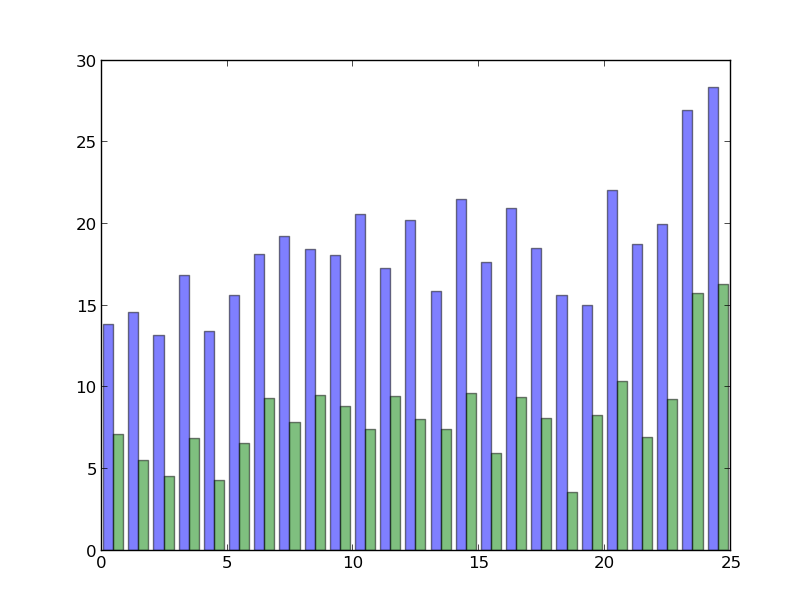
\includegraphics[width=\textwidth]{tr-te-diff_FF-TT}}
\caption{Accuracy differential between training and test as a function of chord class, ordered along the x-axis from most to least common in the dataset for ETD:False (blue) and ETD:True (green) conditions.}
\label{fig:classes}
\end{figure}

One potential cause of over-fitting is due to an under-representation of some chord classes in the dataset.
If this were the case, the most frequent classes should be unaffected by data augmentation, while less common classes would exhibit drastic swings in performance.
Focusing here on Arch:3--1, Figure \ref{fig:classes} shows the change in accuracy between data conditions for both training and test sets as a function of chord class, sorted by most to least common in the dataset.
This plot indicates that, while transposing data during training reduces over-fitting, it does so uniformly across chord classes, on the order of about $10\%$.
Therefore, all chord classes benefit equally from data augmentation, which is characteristic of intra-class variance more so than inadequate data for less common classes.

\begin{figure}[!t]
\centering
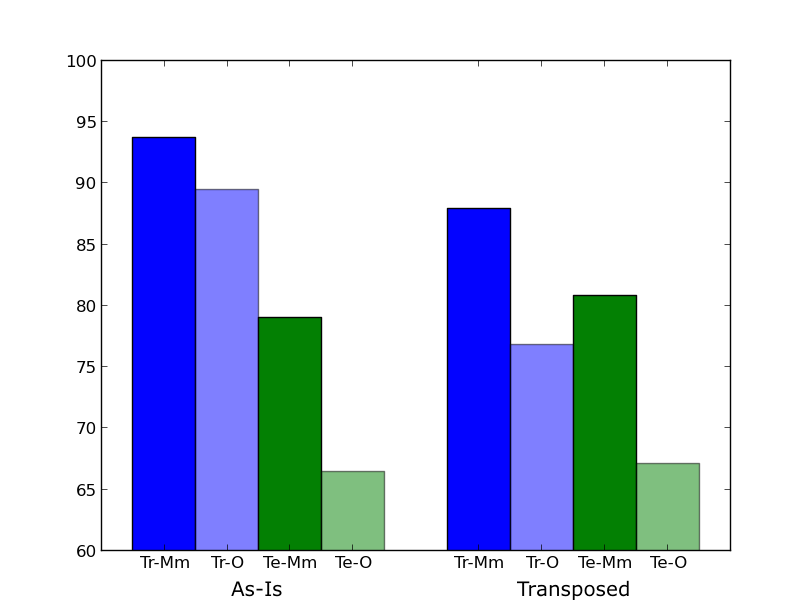
\includegraphics[width=\textwidth]{FF-TT_Mm-vs-other}
\caption{Effects of transposition on classification accuracy as a function explicitly labeled Major-Minor chords (dark bars), versus other chord types (lighter bars) that have been resolved to their nearest Major-Minor equivalent, for training (blue) and test (green) in standard (left) and transposed (right) conditions.}
\label{fig:strict_vs_others}
\end{figure}

If this is indeed the case, there are likely two main sources of intra-class variance: the practice of resolving all chord classes to Major-Minor, or error in the ground truth transcriptions.
As a means to assess the former, Figure \ref{fig:strict_vs_others} plots the accuracy for chords that strictly labeled root-position Major-minor (Mm) versus all other (O) chords that are mapped into these classes in the train (Tr) and test (Te) conditions, with and without transposition.
This is a far more informative figure, resulting in a few valuable insights.
First, there is a moderate drop in performance over the training set for strictly Major-minor chords when data are transposed ($\approx -5\%$), but this causes a noticeable increase in generalization for strictly Major-minor chords in test set ($\approx +3\%$).
Other chords, however, experience a significant decrease in performance within the training set ($\approx -11\%$) with transposition, but register a negligible improvement in the test set ($>1\%$).
One interpretation of this behavior is there is too much conceptual variation in the space of Other chords to meaningfully generalize to unseen data that is also not strictly Major-minor.
This defintion by exclusion gives rise to a class subset that is less populated than its strict counterpart, but will inherently contain a wider range of musical content.
Though a sufficiently complex model may be able to overfit these datapoints in the absence of transposition, counting each observation toward every pitch class distributes the added variance across all classes evenly.
This causes the model to ignore uncommon modes in the class distribution as noise, while reinforcing the strict Major-minor model in the process.

% Additionally, not only is generalization for strict Major-minor chords considerably better than that of Other chords when trained with transposition, but it achieves better recall than Other chords in the training set.
% This means ...

\begin{figure}[!t]
\centering
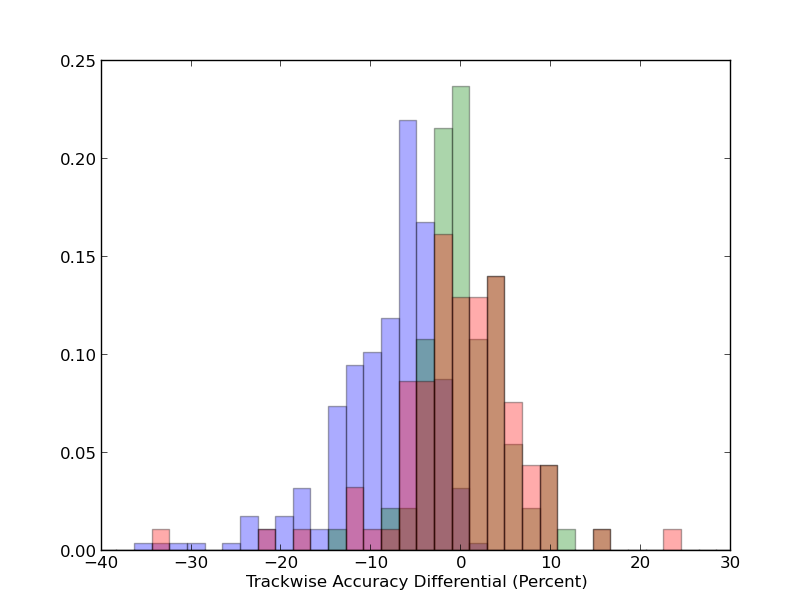
\includegraphics[width=\textwidth]{arch_5-FF_TT_accdiff2}
\caption{Histograms of trackwise recall differential between normal and transposed data conditions, for training (blue), validation (red) and test (green) datasets.}
\label{fig:acc_diff}
\end{figure}

In addition to the effects of vocabulary resolution, there is also a question where this error resides in the data.
To address this point, track-wise histograms of recall differential are computed with and without data transposition for the training, validation, and test splits, shown in Figure \ref{fig:acc_diff}.
Interestingly, performance over most tracks is unaffected or only slightly changed by the transposed data condition, as evidenced by the near-zero mode of the distributions.
Some tracks in the training set, however, result in considerably worse performance when the data is transposed.
This is intuitively satisfying because the repetitive nature of music would cause observations drawn from the same recording to be highly correlated, and therefore multiple instances of rare chords, outliers, or labeling errors should be well localized.
Additionally, this clearly indicates that some tracks are particularly challenging or problematic, and may offer insight into future areas of improvement.

\begin{figure}[!t]
\centering
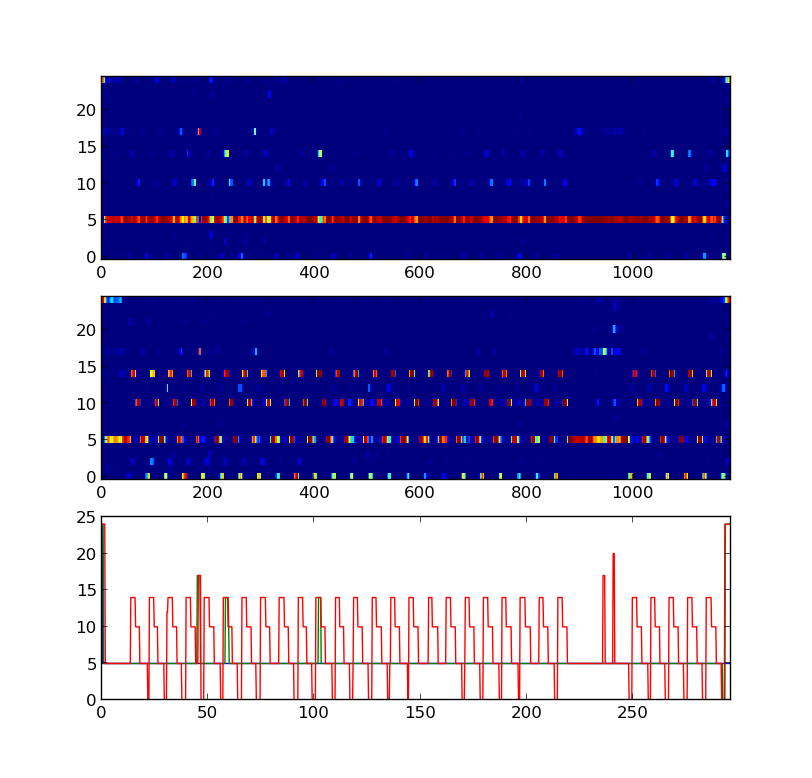
\includegraphics[width=\textwidth]{u2-ff_tt_gtplot}
\caption{.}
\label{fig:u2fu}
\end{figure}

An instance of one such ``problem'' track, ``With or Without You'' by U2, is given in Figure \ref{fig:u2fu}.
Here, the ground truth transcription consists primarily of four chords: \texttt{D:maj}, \texttt{D:maj/5}, \texttt{D:maj6/6}, and \texttt{D:maj(4)/4}.
When resolved to the Major-minor vocabulary, the transcription is reduced entirely to \texttt{D:maj}.
Without transposing data during training, the model is able to call nearly the entire track \texttt{D:maj}; with transposition during training, however, the model is unable to reproduce the ground truth transcription and instead tracks the bass motion, producing \texttt{D:maj}, \texttt{A:maj}, \texttt{B:min}, and \texttt{G:maj}, a very common harmonic progression in popular music.
As far as quantitative evaluation is concerned, this second estimation exhibits a high degree of mismatch with the reference transcription, but is qualitatively reasonable and arguably far more useful to a musician.
Importantly, this illustrates that the process of mapping chords to a reduced vocabulary can cause objective measures to deviate from subjective experience, and thus misleading evaluation.


\subsection{Conclusions}
\label{subsec:conclusions}

Following this initial inquiry, there are a number of conclusions to draw that should influence subsequent work.
First and foremost, the practice of chord name resolution is the largest source of error, both in training and test, as doing so creates multi-modal distributions that can be difficult to model directly.
This challenge stems from the combination of weak conceptual associations between the classes, and diminshed amount of data for the model to discover such diverse relationships.
Therefore, if for this reason alone, future work should consider larger vocabulary chord estimation, as the additional labeling information simplifies the learning problem by encouraging the machine to model different pockets of class densities separately.
Additionally, there is some evidence, in the vein of Figures \ref{fig:acc_diff} and \ref{fig:u2fu}, that chord names with modified intervals or bass information may be a source of noise in the reference chord annotations.
Ignoring over-specified chord names would lead to more stable evaluation while maximizing confidence in the ground truth data.



\section{Large Vocabulary Chord Estimation}
\label{subsec:large_vocabulary_ace}

Combining observations resulting from the previous study with other recent trends in ACE research, the focus now turns to the task of large vocabulary ACE.
There is a small body of research pertaining to vocabularies beyond the Major-minor formulation, but, for the same reasons discussed in \ref{subsec:problem_formulation}, comparing new endeavors to these efforts is problematic due to differences in the vocabularies considered and data used.
Perhaps the most advanced large-vocabulary ACE systems to date is the recent work of Cho \cite{Cho2014}.
The design of this system is largely consistent with the previous overview of ACE research.
A multiband chroma representation is computed from beat-synchronous audio analysis, producing four parallel chroma features.
Each is modeled by a separate Gaussian Mixture Model, yielding four separate observation likelihoods as a function of time.
These four posteriors are then decoded jointly, using a k-stream HMM, resulting in a time-aligned chord sequence.
In addition to being one of the highest performing systems at the recent iteration of MIReX, a software implementation was obtained, thereby enabling direct comparisons with this work.
It also considers the largest vocabulary to date, and presents an even greater challenge to the application of deep learning to ACE.


\subsection{Data Considerations}
\label{subsec:data_considerations}
Following the previous work of Cho \cite{Cho2014}, thirteen chord qualities, given in Table \ref{tab:qualities}, in all twelve pitch classes and one no-chord class are considered here, for a total of 157 chord classes.
Having all four datasets at hand, these collections are merged into the largest collection of chord transcriptions used, totalling 1235 tracks.
Given that the collections were curated in isolation of each other, it is a necessary first step to identify and remove duplicates to avoid data contamination during cross validation.
To these ends, each recording is checked against the EchoNest Analyze API\footnote{\url{http://developer.echonest.com/docs/v4}} and associated with its track and song identifiers, corresponding to the recording and work, respectively.
Though multiple track IDs will map to the same song ID, uniqueness is defined at the level of a song to ensure duplicates are removed.
This identifies 18 redundant songs, and all but one is dropped from the total collection, resulting in a final count of 1217 unique tracks.

Based on conclusions of the pilot study, the decision is made to ignore all chord labels that do not strictly match one of the considered qualities, i.e. chords that specify interval modifications, e.g. \texttt{A:min(*b3)}, or non-root inversions, e.g. \texttt{C:maj/5}.
The motivation for doing so is two-fold.
First, the increased number of chord qualities makes it difficult to map certain chords into one class or another, such as \texttt{D:sus4(b7)}, which sits halfway between a \texttt{D:sus4} and a \texttt{D:7}.
Second, cleaning the reference data on this criteria can only improve annotation consistency; considering that the cumulative data is compiled from multiple sources and several dozen annotators over the course of a decade, it is quite unlikely that such nuanced conventions were used identically by all subjects involved.
This ignored subset comprises only a small percentage of the overall data, and helps filter out suspicious chord spellings, such as \texttt{D:maj(\*1)/$\sharp$1} or \texttt{A:maj(2,\*3)/2}.

% Statistics
Unsurprisingly, as the data is collected from real music, the distribution of absolute chord classes is extremely imbalanced.
In fact, some chord qualities do not occur in every root, and stratifying the data for training, validation, and testing only exacerbates the issue.
Much previous work, including the previous discussion, has demonstrated that chord names can be rotated to distribute instances across qualities, rather than absolute classes, motivating root-invariant analysis.
A root-invariant histogram of the chord qualities contained in the merged dataset, given in Figure \ref{fig:training_distribution}, clearly shows there is severe relative and absolute class imbalance.
To the former, a stark division exists between the majority classes (\texttt{maj}, \texttt{min}, \texttt{maj7}, \texttt{min7}, \texttt{7}, and \texttt{N}), and the minority classes (\texttt{maj6}, \texttt{min6}, \texttt{dim}, \texttt{aug}, \texttt{sus4}, \texttt{sus2}, \texttt{dim7}, \texttt{hdim7}).
The ratio, for example, between the most and least common qualities, \texttt{maj} and \texttt{dim7} respectively, is nearly three orders of magnitude ($\approx 700$).
Arguably, the more challenging imbalance is an overall lack of data for some minority classes.
Over all roots, the total duration of \texttt{dim7} is on the order of hundreds of seconds.
Considering the repetitive structure of music, it is reasonable to assume that these few instances also occur in the same small number of tracks, limiting the variability of this data.

\begin{figure}[!t]
\centering
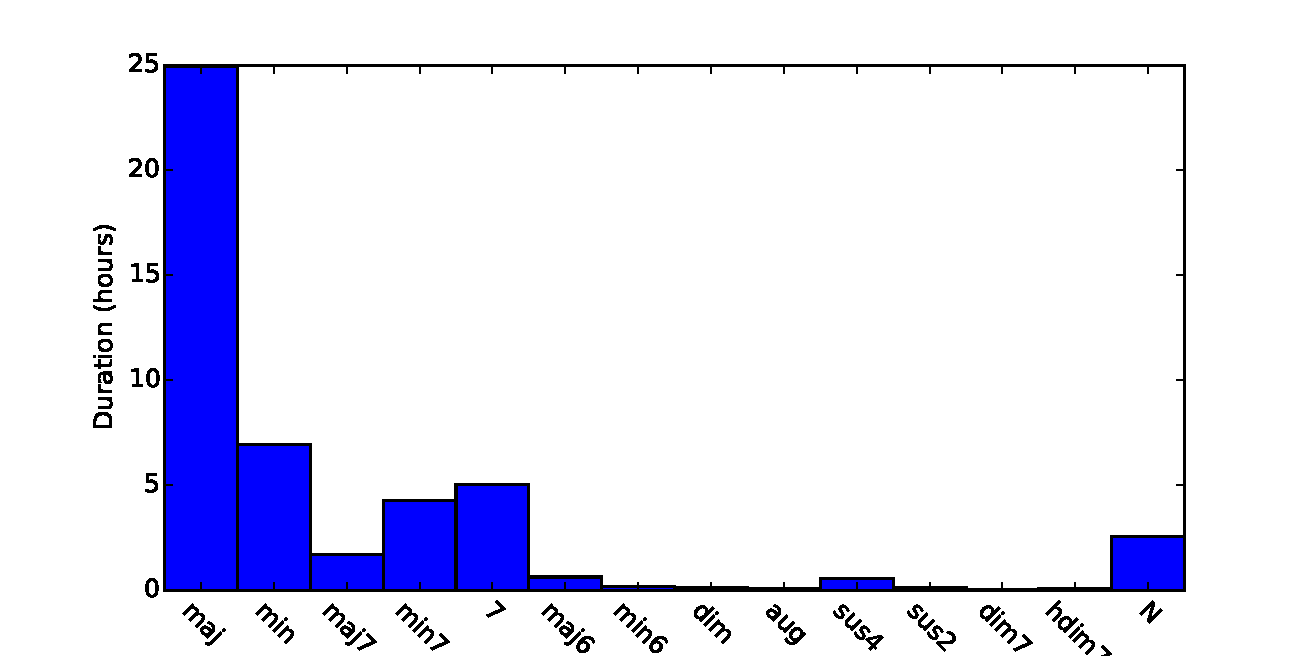
\includegraphics[width=\textwidth]{training_distribution}
\caption{Histogram of chord qualities in the merged data collection.}
\label{fig:training_distribution}
\end{figure}


\subsection{Experimental Setup}
\label{subsec:experimental_setup}
This work proceeds directly from the previous study, and takes a similar approach in many facets.
There are a handful of important distinctions to make between the two, however, and these differences are detailed here.

\subsubsection{Input Representation}
\label{subsubsec:data_considerations}
A comparable constant-Q transform is applied to the audio at a framerate of 20Hz, without subsequent low-pass filtering or decimation, and time-frequency patches are formed from 20 frames, corresponding to 1 second.
Whereas the previous study aimed to learn context directly, there is the inherent concern that a low input framerate will reduce the amount of data available for training beyond what is required by the model.
In lieu of learning this context, standard post-filtering will be applied in the form of a uniform-transition HMM with a tunable self-transition penalty, consistent with \cite{Cho2014PhD}; this is introduced in greater detail shortly, in \ref{subsubsec:viterbi}.

Additionally, local contrast normalization is included as a standard preprocessing stage, with minor modifications.
In previous work, a threshold is placed on the scaling term given by the average standard deviation over the entire input.
While this may be suitable in the field of computer vision, where spatial dimensions are equivalent in 2-space, audio data behave differently in time and frequency.
Namely, complex sounds often exhibit an overtone series, and energy becomes more densely concentrated in higher frequencies.
This can have the undesirable effect of inadequately gaining regions that are more sparse.
To correct for this behavior, the scaling coefficient is adjusted such that the frequency range considered is a piecewise function of frequency height, defined as follows:

\begin{align*}
X_filt = (X \circledast W) \\
V = X_filt - X \\
S_k = V \circledast W_k \\
S_k = max(S_k, \mu_{S_k}) \\
Y = \sum_{k=0}^{K-1} g_k * \frac{V}{S_k} \\
\end{align*}

\noindent To illustrate the benefit of this piecewise combination, an example track is given in Figure \ref{fig:lcn_mods}, both with and without the octave-dependent modification.

\begin{figure}[!t]
\centering
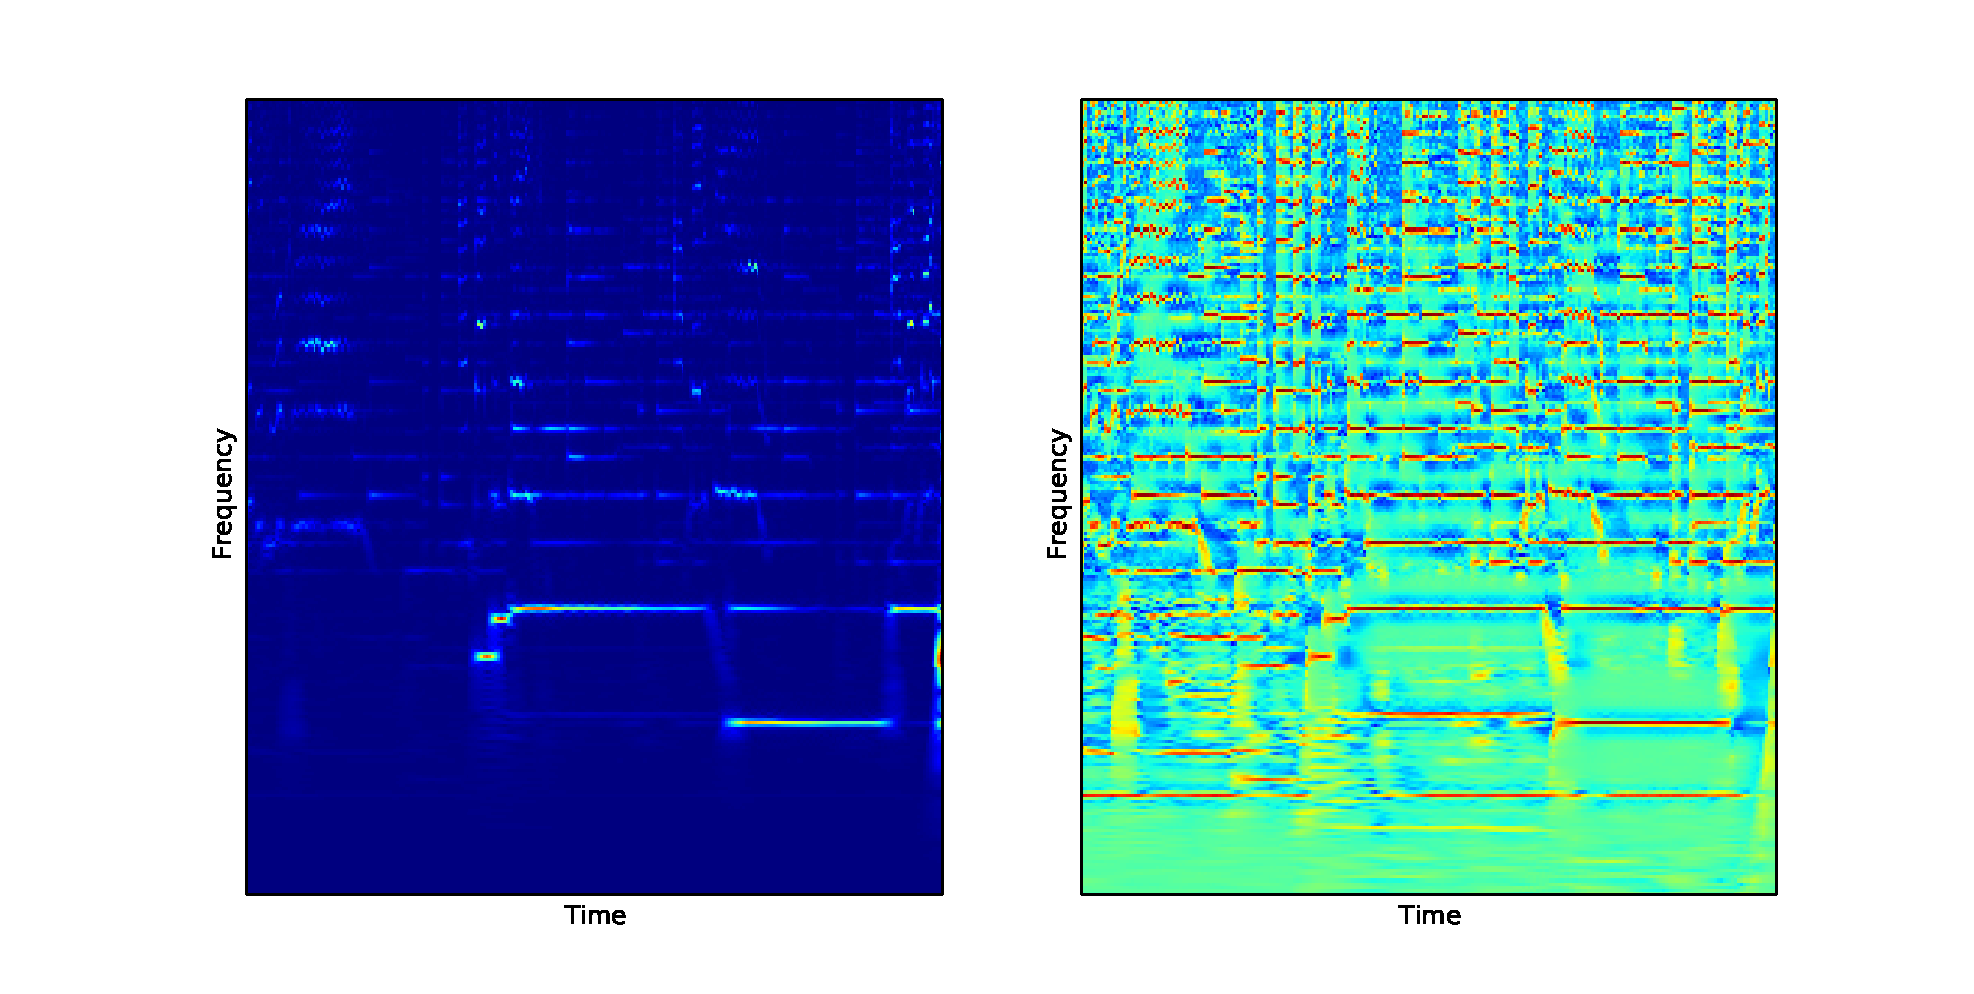
\includegraphics[width=\textwidth]{cqt_compare}
\caption{The visible effects of octave-dependent LCN, before (left) and after (right).}
\label{fig:lcn_mods}
\end{figure}


\subsubsection{Designing a Root-Invariant Classifier}
\label{subsubsec:root_invariance}
One of the key findings from the previous study of deep networks for ACE, consistent with previous research, is the importance of enforcing or encouraging root-invariance in the model.
With GMMs, this is typically achieved by rotating all data, i.e. chroma features, to the same root and fitting a model for each quality.
Then, when applying the model, likelihoods are estimated for each root by circularly rotating chroma through all twelve positions to recover the full space of chord classes.
In the pilot study on chord estimation, this concept was mimicked by rotating the data in the input domain.
While it led to improved results, rotating the data is less than ideal for at least two reasons.
One, it is an implicit, rather than explicit, association between classes, and the model is tasked with learning redundant relationships.
During training, the model needs to learn the same behavior 12 times over to represent each quality in every root.
Two, rotating data in the input space may create unnatural artifacts in the kinds of data the model learns to expect, and it is not clear what, if any, side effects this may have.
It is assumed that this does not fundamentally change the latent distribution of the data used for training, but it may cause a mismatch with real data at test time.

An alternative to rotating the data, as convolutional networks have amply demonstrated, is to build the invariance directly into the architecture.
This is realized here by defining a four layer network composed entirely of convolution operations, such that the classifier's weights for each quality are shared over all roots; a diagram of this configuration is given in Figure \ref{fig:fullconvnet}.
Simplifying conceptually, this proceeds as follows: the penultimate representation is designed to yield a matrix with shape $(12 \times N)$, corresponding to the number of pitch classes and the chosen output dimensionality of the second to last layer, respectively; the chord classifier is then applied by taking the inner product with a weight matrix with shape $(N \times 13)$, corresponding to the dimensionality of the previous layer and the number of chord qualities, respectively.
For ease and efficiency this is implemented as a convolution, but the result is equivalent.
This produces a $(12 \times 13)$ matrix, which is flattened to represent the 13 qualities in all possible roots.

Note that the no-chord class is not captured by this operation, however, and a separate fully connected layer is applied in parallel to the flattened penultimate representation to estimate this class independently.
This one-dimensional no-chord estimator is then concatenated with the flattened chord estimator, and this combined representation of 157 classes is normalized by the softmax operation to yield the probability mass function over all classes.

\begin{figure}[!t]
\centering
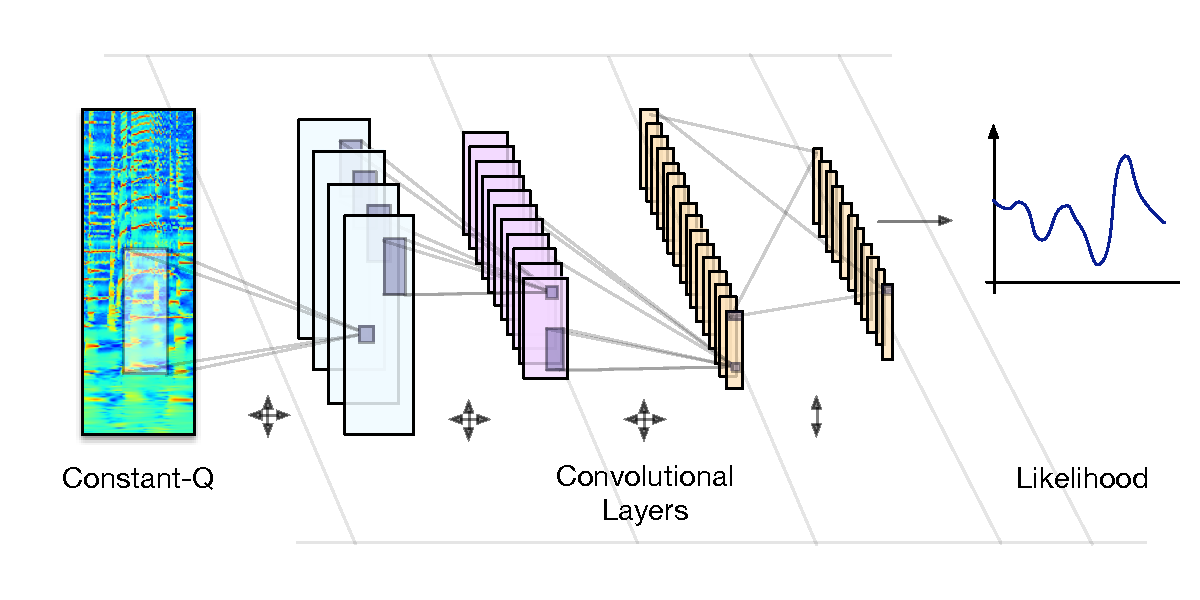
\includegraphics[width=\textwidth]{fullconvnet}
\caption{A Fully Convolutional Chord Estimation Architecture.}
\label{fig:fullconvnet}
\end{figure}

\subsubsection{Convolutional Dropout}
\label{subsubsec:conv_dropout}

Here, the principles of dropout, discussed in Chapter \ref{chp:deep_learning}, are extended to 3D convolutions.
In the weight-matrix case, training with dropout effectively ignores activations of an transformed output, setting them to zero.
Considering each output coefficient as a measure of activation for a given ``feature'', the act of dropout can be interpretted as sub-sampling the feature extractors learned by the model.

By extension, there are two ways the same principle could be applied in the case of 3D convolutions: over an entire 3D kernel, or distributed among all 2D receptive fields among all kernels.
We opt for the former as a trade-off in the degree of randomness dropout introduces to the training processes; the merits of one approach over another are left for future work.
Expressed formally, the $i^{th}$ kernel, $W_i$, can be masked with probability $p$, resulting in the possibly empty feature map, $Z_i$:

\begin{equation}
% \label{eq:conv_dropout}
Z_i = binomial(p) * h(X \circledast W_i + b_i) / (1.0 - p)
\end{equation}

\noindent where the output is also scaled by the complement of the probability.
Here, it is expected that each kernel learns a collection of feature extractors that, on average, work well together.
In the language of coadaptation, the tensor can be seen as a ``team'' of feature detectors, and as such correlations are broken up at this mid, as opposed to global, level.

There are two small implementation details worth noting.
First, the same parameters in the model are dropped out over the entire batch, and not separately for each datapoint in the batch.
In the bagging and model selection interpretation of dropout, this is analagous to updating one different model at each update step; the alternative effectively updates several models simultaneously.
Again, future work is necessary to determine the advantages of one approach versus another, but the single-select approach is preferred for its parallels to coordinate block descent \cite{somebody}.
Additionally, the original proposal of dropout suggests that the activations of all outputs be halved when using the full model at test time.
This is somewhat cumbersome in practice, and, as indicated in Eq. (\ref{eq:conv_dropout}), scale \emph{up} the parameters during training, allowing models in test to be agnostic of dropout.


\subsubsection{Architectural Considerations}
\label{subsubsec:arch}

Given the theoretical relationship between dropout and model averaging, it is reasonable to expect that larger dropout ratios will necessitate larger architectures.
Therefore, a variety of model complexities are explored by changing the number of number of kernels in each layer; the primary weight shapes of the networks are given in Table \ref{tab:lvce_archs}:

\begin{table}[t]
\begin{center}
\caption{Parameter shapes in the three model complexities considered.}
\label{tab:lvce_archs}
\begin{tabular}{l | c | c | c | c }
layer & L & XL & XXL & pooling\\
\hline
0   & (16,  1, 5, 13) & (20,  1, 5, 13) & (24,  1, 5, 13) & (2, 3) \\
1   & (32, 16, 5, 37) & (40, 20, 5, 37) & (48, 24, 5, 37) & (2, 1) \\
2   & (64, 32, 1, 33) & (80, 40, 1, 33) & (96, 48, 1, 33) & (2, 1) \\
3.a & (13, 64, 1,  1) & (13, 80, 1,  1) & (13, 96, 1,  1) &   --   \\
3.b &    (768, 1)     &     (960, 1)    &    (1152, 1)    &   --   \\
\hline
\end{tabular}
\end{center}
\end{table}

The first four layers are 3D-convolutions, and thus the weights are 4 dimensional, corresponding to the number of kernels, the number of input feature maps, filter size in the time dimension, and filter size in the frequency dimension, respectively.
The first three of these layers make use of max-pooling in time by a factor of 2, but only the first also performs max-pooling in frequency, by a factor of 3.
As before, downsampling in frequency is performed in the spirit of learning slight tuning invariance, consistent with 12-TET.
The final layer, 3.b, corresponds to the fully-connected no-chord regressor, and the shape of this weight matrix is given as the input and output dimensionalities, respectively.


\subsubsection{Correcting Class Biases with Scaled Likelihood Estimation}
\label{subsubsec:scaled_likelihood_estimation}
Having defined the output of the model as a probability function, it is trivial to again optimize the parameters to the negative log-likelihood over the dataset.
However, there are two difficulties that prohibit the uniform presentation of classes, as in previous work.
First, due to the increased number of classes, minibatches would either need to consist of many datapoints, increasing the processing time of each batch, or the learning rate would need to be smaller or diminishing over time to prevent oscillation, increasing the number of iterations necessary to converge.
To the latter point, it is easy to imagine scenarios where gradient descent wobbles back and forth between updates, as each batch pulls the parameters in a slightly different direction.
The other challenge this raises is a result of the considerable class imbalance, where uniform presentation would spend too much time on minority classes, while slowly the full extent of the majority classes.

The solution to this problem is found in Bayes' theorem, where the network is understood as yielding a class posterior probability, $P(Y|x)$, for the chord class, $Y$, given the observation, $x$:

\begin{equation}
P(x|Y) = \frac{P(Y|x)*P(x)}{P(Y)}
\end{equation}

The observation likelihood, $P(x|Y)$, is then a function of the posterior, the class prior, $P(Y)$, and probability of the observation itself, $P(x)$.
This final quantity is independent and thus can be ignored:

\begin{equation}
P(Y|X) \varpropto \frac{P(X|Y)}{P(Y)}
\end{equation}

While the deep network is trained to produce the class posterior, the class prior can be measured empirically over the training set, and divided out after the fact.
Referred to as \emph{scaled likelihood estimation}, this strategy has proven effective at reducing the effects of class imbalances in the functionally related domain of automatic speech recognition \cite{Deng, others}.
Notably, scaled likelihood estimation is particularly attractive here because it scales well with the number of estimated classes.

As a final comment, a possible pitfall when applying likelihood scaling is a matter of numerical stability arising from the least represented classes, or classes that might not even occur in the training set.
Whereas this can be mitigated with pseudo-counting \cite{?} --setting an heuristically determined, non-zero lower bound-- the class prior here is computed by counting each observation toward the same quality in all roots.
Though this prior could be seen as a coefficient vector to optimize in a more direct way, this approach works reasonably well in practice.


\subsubsection{Training and Early Stopping}
\label{subsubsec:early_stopping}

In contrast to the previous study, which converged to a stable result in a few thousand iterations, it takes considerably more effort to train models for this task, on the order of hundreds of thousands of iterations.
Given the lengthy run time, parameters are checkpointed every 1k iterations during training, and frame the problem of early stopping as a brute-force search over a finite set of parameter configurations.
Due to the application of Viterbi and the coupling with the self transition penalty, validation is non-trivial and computationally expensive.
Therefore, exhaustive validation is performed every 10k iterations, starting at 5k.
The best model and self-transition penalty are chosen by finding the configuration with the highest harmonic mean over all evaluation metrics given in Section \ref{subsec:eval_methodology}.


% \subsubsection{Viterbi Post-filtering}
% \label{subsubsec:viterbi}

% Though somewhat standard at this point in ACE research, it is worthwhile to properly formalize the HMM-based post-filtering approach used here, given its considerable impact on system performance.


% \subsection{Research Questions}
% \label{subsec:research_questions}

% What can we do to overcome these issues of class imbalance?
% % Build class invariance into the model
% % use dropout during training
% % smaller inputs, more constraints, leverage HMM for context / stabilization
% How does the deep learning system compare to the state of the art?
% % Beats it! depending on who you ask, at least
% What are the advantages and challenges of training with larger vocabularies?
% % Resolve predictions back to maj / min, how does it do? Should be better...
% % Larger vocabularies result in more class collisions
% % But this is actually a manifestation of ambiguity
% Does observed system behavior correspond to quantitative evaluation?
% % Getting a lot of reasonable confusions.
% % Maybe this is a function of an inherently subjective task.
% % The ground truth data on hand were ``reviewed'', and there are no records concerning which chord names may have been contested or corrected.
% % Rock corpus


\subsection{Experimental Results}
\label{subsec:quantitative_results}


\begin{table}[t]
\scriptsize
\begin{center}
\caption{Micro-recall across metrics for over the training data.}
\label{tab:recall_train}
\begin{tabular}{cc|rrrrrrr}

\hline
 \multicolumn{2}{c|}{Model} &   triads &   root &  mirex &   tetrads &   sevenths &   thirds &   majmin \\
\hline
\hline
\multicolumn{2}{c|}{Cho, 2014} &   0.8053 & 0.8529 &  0.8205 &    0.6763 &     0.6823 &   0.8261 &   0.8109 \\
\hline
 L &  0.0 & 0.9087 & 0.9249 &  0.9140 & 0.8600 & 0.8601 &   0.9177 &   0.9097 \\
 & 0.125 &   0.8706 & 0.9018 &  0.8785 &    0.7798 &     0.7792 &   0.8895 &   0.8718 \\
 &  0.25 &   0.8382 & 0.8811 &  0.8490 &    0.7266 &     0.7277 &   0.8637 &   0.8405 \\
 & 0.5 &   0.7916 & 0.8491 &  0.8079 &    0.6577 &     0.6641 &   0.8262 &   0.7970 \\
\hline
  XL &   0.0 &   0.9236 & 0.9353 &  0.9277 &    0.8903 &     0.8906 &   0.9300 &   0.9244 \\
   &  0.125 &   0.8899 & 0.9145 &  0.8962 &    0.8217 &     0.8214 &   0.9049 &   0.8908 \\
   &  0.25 &   0.8504 & 0.8888 &  0.8610 &    0.7374 &     0.7385 &   0.8734 &   0.8527 \\
   &  0.5 &   0.7972 & 0.8541 &  0.8118 &    0.6632 &     0.6683 &   0.8329 &   0.8014 \\
\hline
  XXL &  0.0 &   0.9462 & 0.9528 & 0.9487 &    0.9297 &     0.9300 &   0.9498 &   0.9466 \\
   &   0.125 &   0.8994 & 0.9209 &  0.9048 &    0.8386 &     0.8374 &   0.9133 &   0.8997 \\
   &   0.25 &   0.8701 & 0.9041 & 0.8777 &    0.7833 &     0.7828 &   0.8921 &   0.8710 \\
   &   0.5 &   0.8043 & 0.8573 &  0.8184 &    0.6783 &     0.6820 &   0.8374 &   0.8080 \\
\hline
\end{tabular}
\end{center}
\end{table}

Following from the setup defined above, the three model complexities --X, XL, and XXL-- are trained with four dropout values, $p_{dropout} \in \{0.0, 0.125, 0.25, 0.5\}$ across five folds of the data.
Note that when $p_{dropout} = 0.0$, this is equivalent to training a model without dropout.
Additionally, the system presented in \cite{Cho2014PhD}, referred to here simply as ``Cho'', is trained on identical partitions of the data and evaluated alongside the deep networks.
Micro-recall for the various comparison functions, averaged across folds, is given in Tables \ref{tab:recall_train} and \ref{tab:recall_test} for the training and test splits, respectively.


\begin{table}[t]
\scriptsize
\begin{center}
\caption{Micro-recall across metrics for over the holdout (test) data.}
\label{tab:recall_test}
\begin{tabular}{cc|rrrrrrr}

\hline
\multicolumn{2}{c|}{Model}  & triads &   root &   mirex &   tetrads &   sevenths &   thirds &   majmin \\
\hline
\hline
\multicolumn{2}{c|}{Cho, 2014} &   0.7970 & 0.8475 &  \textbf{0.8147} &    0.6592 &     0.6704 &   0.8197 &   0.8057 \\
\hline
L & 0.0 &   0.7939 & 0.8442 &  0.8102 &    0.6583 &     0.6725 &   0.8135 &   0.8041 \\
  & 0.125 &   0.7951 & 0.8465 &  0.8109 &    0.6516 &     0.6616 &   0.8203 &   0.8028 \\
 & 0.25 &   0.7882 & 0.8445 &  0.8039 &    0.6509 &     0.6592 &   0.8175 &   0.7950 \\
  & 0.5 &   0.7762 & 0.8372 &  0.7936 &    0.6358 &     0.6442 &   0.8115 &   0.7832 \\
\hline
 XL &   0.0 &   0.7939 & 0.8432 &  0.8098 &    0.6589 &     0.6736 &   0.8122 &   0.8042 \\
  &  0.125 &   \textbf{0.7995} & 0.8493 &  0.8145 &    \textbf{0.6673} &     \textbf{0.6788} &   0.8227 &   \textbf{0.8077} \\
  &  0.25 &   0.7950 & 0.8479 &  0.8114 &    0.6493 &     0.6580 &   0.8215 &   0.8023 \\
  &  0.5 &   0.7773 & 0.8401 &  0.7940 &    0.6351 &     0.6430 &   0.8147 &   0.7836 \\
\hline
   XXL & 0.0 &   0.7969 & 0.8463 &  0.8130 &    0.6583 &     0.6741 &   0.8136 &   0.8080 \\
   &  0.125 &   0.7993 & 0.8477 &  0.8140 &    0.6633 &     0.6745 &   0.8215 &   0.8075 \\
   &  0.25 &   0.7947 & \textbf{0.8497} &  0.8092 &    0.6592 &     0.6686 &   \textbf{0.8241} &   0.8020 \\
   &  0.5 &   0.7768 & 0.8369 &  0.7941 &    0.6392 &     0.6468 &   0.8121 &   0.7830 \\
\hline
\end{tabular}
\end{center}
\end{table}

There are several observations that may be drawn from these two tables.
First, in the absence of dropout, the deep network models considered here are able to overfit the training data.
This is an important finding in so far as making sure that the fully-convolutional architecture is not overly constrained, and indicates that the XXL model is a reasonable upper bound on complexity.
The effect of dropout on performance over the training set is significant, as it reduces overfitting consistent with increased values.

Shifting focus to performance on the test set, it is obvious that these differences in training set performance have little impact on generalization, and all models appear to be roughly equivalent.
A small amount of dropout --0.125 or 0.25-- has a slight positive effect on generalization; too much dropout, on the other hand, seems to have a negative effect on performance.
There are two possible explanations for this behavior:
one, a high degree of convolutional dropout is more destabilizing than in the fully-connected setting;
and two, these models were not finished learning, and stopped prematurely.

Overall, the best deep networks appear to be essentially equivalent to the state of the art comparison system; XL-0.125 just barely eclipses ``Cho'' in every metric but ``mirex'', while XXL-0.25 is right on its heels.
The different metrics indicate that confusions at the strict level are predominantly musically related, i.e. descending in order from root, thirds, triads, sevenths, tetrads.
Interestingly, the performance gap between the ``root'' and ``triads'' scores is quite small, $\approx 5\%$, while the gap between ``root'' and ``tetrads'' is nearly $20\%$, for all models considered.
One way to interpret this result is that these systems are quite robust in the estimation of three-note chords, but struggle to match the way in which reference annotators use sevenths.


\begin{table}[t]
\begin{center}
\caption{Quality-wise macro-recall statistics.}
\label{tab:qwise_macro_recall}
\begin{tabular}{l|rrrr}
\hline
 train   &    0.0 &   0.125 &   0.25 &    0.5 \\
\hline
 L       & 0.8858 &  0.8263 & 0.7403 & 0.5838 \\
 XL      & 0.9049 &  0.8569 & 0.7652 & 0.6147 \\
 XXL     & 0.9421 &  0.8838 & 0.8232 & 0.6459 \\
\hline
 test   &    0.0 &   0.125 &   0.25 &    0.5 \\
\hline
 L      & 0.4306 &  0.5029 & 0.5240 & 0.5135 \\
 XL     & 0.4174 &  0.4887 & \textbf{0.5281} & 0.5253 \\
 XXL    & 0.3935 &  0.4825 & 0.5127 & 0.5257 \\
\hline
\end{tabular}
\end{center}
\end{table}

Moving on, the results for the quality-wise macro-recall, or average chord quality accuracy, is given in Table \ref{tab:qwise_macro_recall}.
While dropout again able to considerably reduce overfitting in the training set, it appears to have a more profound effect here towards generalization.
Whereas before a 0.5 dropout ratio seemed to result in the ``worst'' deep networks, here it leads to the best generalization across all chord qualities.
Furthermore, the best performing models, according to micro-recall, are not the best performing models in this Table.
Thus these results allude to the notion that micro-recall over all data may have an inverse relationship with quality-wise macro-recall.


\begin{table}[t]
\begin{center}
\scriptsize
\caption{Individual chord quality accuracies for the XL-model over test data, averaged across all folds.}
\label{tab:ind_qwise_macro}
\begin{tabular}{l|ccccc|c}
\hline
    &   support (min) &    0.0 &   0.125 &   0.25 &    0.5 & Cho, 2014\\
\hline
 C:maj     &  397.4887 & 0.7669 &  0.7390 & 0.6776 & 0.6645 & 0.7196\\
 C:min     &  105.7641 & 0.5868 &  0.6105 & 0.6085 & 0.6001 & 0.6467\\
 C:7       &   68.1321 & 0.4315 &  0.5183 & 0.5783 & 0.5362 & 0.5959\\
 C:min7    &   63.9526 & 0.4840 &  0.5263 & 0.5954 & 0.5593 & 0.5381\\
 N         &   41.6994 & 0.7408 &  0.7679 & 0.7875 & 0.7772 & 0.5877\\
 C:maj7    &   23.3095 & 0.5802 &  0.6780 & 0.7268 & 0.7410 & 0.6587\\
 \hline
 C:sus4    &    8.3140 & 0.2380 &  0.3369 & 0.3811 & 0.4231 & 0.3894\\
 C:maj6    &    7.6729 & 0.1929 &  0.2908 & 0.3847 & 0.3540 & 0.3028\\
 C:sus2    &    2.4250 & 0.1921 &  0.3216 & 0.3698 & 0.3995 & 0.1993\\
 C:dim     &    1.8756 & 0.4167 &  0.4105 & 0.4140 & 0.3955 & 0.5150\\
 C:min6    &    1.5716 & 0.2552 &  0.3870 & 0.4505 & 0.5076 & 0.3129\\
 C:aug     &    1.2705 & 0.3730 &  0.5078 & 0.5346 & 0.5521 & 0.3752\\
 C:hdim7   &    1.1506 & 0.3840 &  0.5688 & 0.6659 & 0.6140 & 0.4593\\
 C:dim7    &    0.5650 & 0.2012 &  0.1790 & 0.2186 & 0.2296 & 0.0643\\
 \hline
 total & -- & 0.4174 &  0.4887 & 0.5281 & 0.5253 & 0.4546 \\
\hline
\end{tabular}
\end{center}
\end{table}

To further assess this claim, the individual chord quality accuracies are broken out by class for ``XL-0.125'', and compared alongside ``Cho'', given in Table \ref{tab:ind_qwise_macro}.
Immediately obvious is the influence of sharp distribution effects in generalization.
Performance for the majority chord qualities, in the upper half of the table, is noticeably higher than the minority classes, in the lower half.
The one exception is that of dominant 7 chords, which seems relatively low, especially compared to ``Cho'';
this is likely a result of V vs V7 confusions, but the annotations do not easily provide this functional information to validate the hypothesis\footnote{The Billboard dataset \emph{does} provide tonic information, and thus this relationship could be recovered from the data; however, it is left here as a fertile area for future work}.
XXL-0.25 yields near identical micro statistics to TMC, but achieves a significant increase in QW macro-recall, 0.5127 to 0.4546 (0.0581).


Notably, the only chord quality to decrease in accuracy with dropout is major, indicating that, with the addition of dropout, the decision boundary between major and its related classes, e.g. major 7 and dominant 7, shift.
However, because of the significant imbalance in the support of each quality, given here in minutes, a small drop in accuracy for major yields a considerable drop in micro-recall overall.
To illustrate, between the 0.125 and 0.25 dropout ratios, major accuracy drops 6\%, while dominant 7 and major 7 accuracy increase 6\% and 5\%, respectively.
In terms of overall time though, this comes at the expense of 24 minutes of major now being classified ``incorrectly'', compared to a combined 5 minutes of dominant and major 7's now being ``correct''.
Therefore, it seems there is a trade-off between these two measures, and thus the representational power of the model does not really change.
Rather, the decision boundaries between overlapping classes must prefer one over the other, and thus model selection may ultimately be a function of use-case.
For example, is it better to have a model that predicts simpler chords, i.e. major, most of the time? Or to have a model that makes use of a wider vocabulary of chords?
Lastly, it is necessary to recognize that, while this quality-wise macro-recall statistic provides a glimpse into more nuanced system behavior, the severe class imbalance results in a rather volatile metric.


% Consider how the algorithms agree with each other
\begin{table}[t]
\begin{center}
\scriptsize
\caption{Micro-recall scores for the two algorithms against each other, and the better match of either algorithm against the reference.}
\label{tab:algo_vs_algo}

\begin{tabular}{lrrrrrrr}
\hline
         &   triads &   root &   mirex &   tetrads &   sevenths &   thirds &   majmin \\
\hline
 DNN vs Cho &   0.7835 & 0.8406 &  0.8044 &    0.6769 &     0.7072 &   0.8148 &   0.8095 \\
 Cho vs DNN &   0.7835 & 0.8406 &  0.8044 &    0.6770 &     0.6982 &   0.8148 &   0.8035 \\
 \hline
 Ref. vs (DNN | Cho) &   0.8243 & 0.8705  &  0.8402  &   0.7037   &   0.7157  &  0.8452  &  0.8331 \\
\hline
\end{tabular}
\end{center}
\end{table}

As a final investigation of algorithm performance with this particular collection of data, having the estimations of two very different computational systems affords the opportunity to explore where they do or do not agree.
Table \ref{tab:algo_vs_algo} contains the micro-recall statistics comparing algorithmic estimations, from ``XL-0.125'' and ``Cho'', against each other, as well as the best track-wise match between either and the reference;
this latter condition is similar in concept to model averaging, and serves to further highlight differences between estimations.
It is interesting to consider that, despite nearly equivalent performance on the metrics reported above, these two systems agree roughly to the same extent either matches the reference annotations.
The conclusion to draw from this is that the errors made by one system are typically different than those of the other.
Therefore, in considering the logical-OR of these estimations, it is clear that the ground truth chord label is often produced by one of the systems, perhaps encouraging the exploration of ensemble methods in future work.


\begin{figure}[t]
\centering
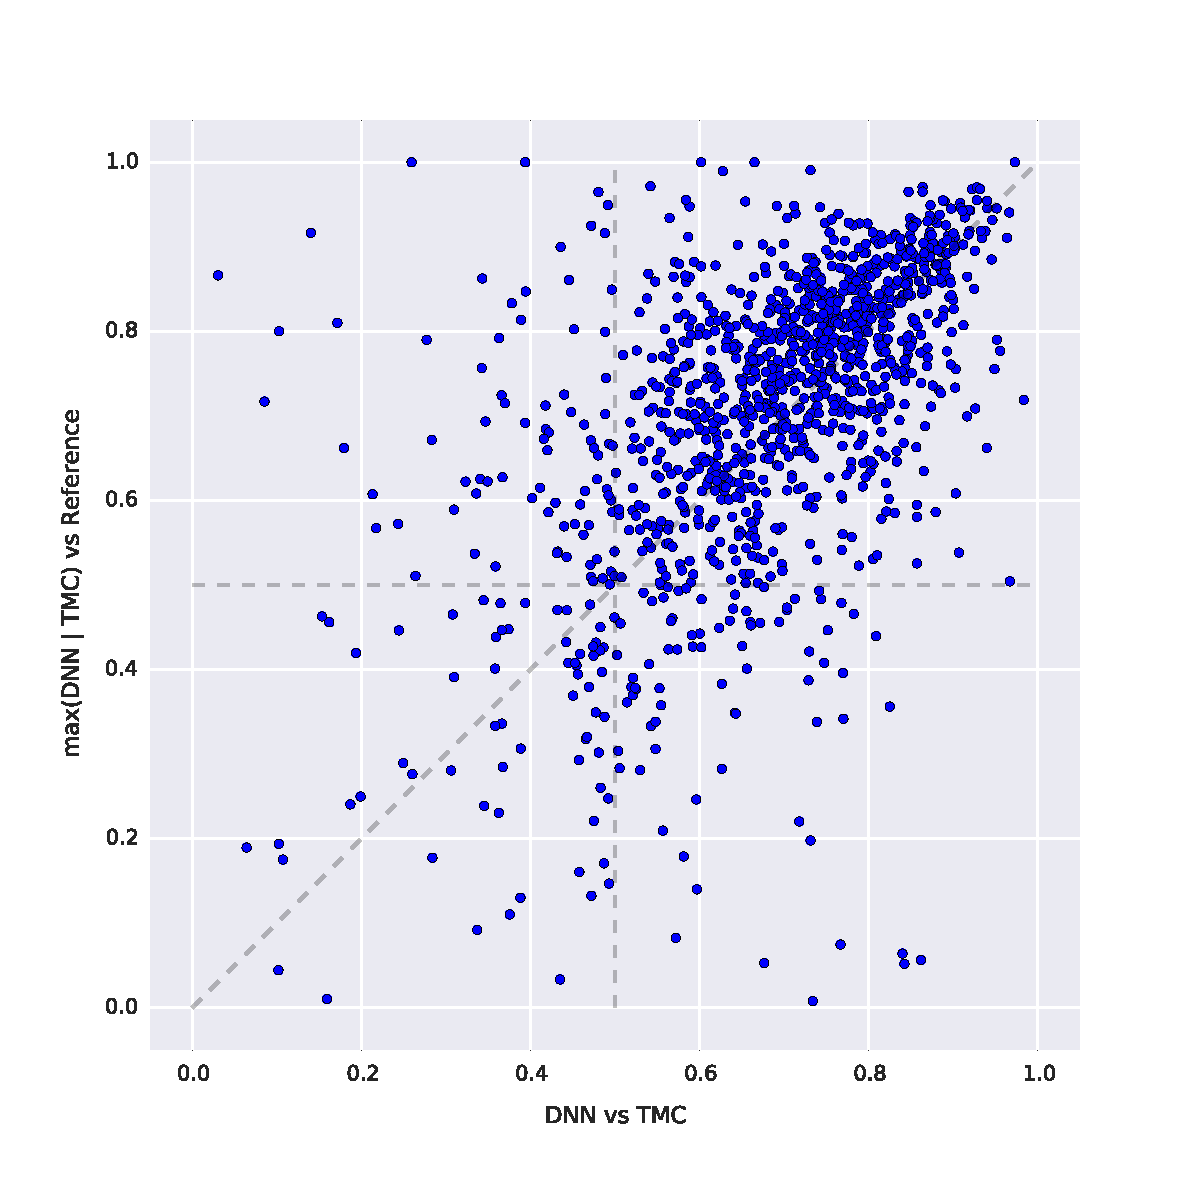
\includegraphics[width=\textwidth]{trackwise_test_agreement}
\caption{Trackwise agreement between algorithms versus the best match between either algorithm and the ground truth data.}
\label{fig:trackwise_test_agreement}
\end{figure}


Expanding on this analysis, it is of considerable interest to compare scores between algorithms versus the best match with the reference on a trackwise basis; this is given in Figure \ref{fig:trackwise_test_agreement} for the ``tetrads'' metric.
Here, each track is represented as a point in coordinate space, with algorithmic agreement along the $x$-axis and best agreement with the ground truth annotations along the $y$-axis.
For clarity, this scatter plot can be understood in the following way:
the line $x=y$ corresponds to an equal level of agreement between all three chord transcriptions;
bisecting the graph horizontally and vertically yields four quadrants, enumerated I-IV in a counterclockwise manner, starting from the upper right.
Tracks that fall in each quadrant correspond to a different kind of behavior.
Points in quadrant I indicate that both estimations and the reference have a high level of agreement ($x > 0.5$, $y > 0.5$).
Quadrant II contains tracks where the algorithms disagree significantly ($x < 0.5$), but one estimation matches the reference well ($y > 0.5$).
Tracks in quadrant III correspond to the condition that no transcription agrees with another, ($x < 0.5$, $y < 0.5$), and are particularly curious.
Finally, quadrant IV contains tracks where the algorithms estimate the same chords ($x > 0.5$), but the reference disagrees with them both ($y < 0.5$).

With this in mind, three-part annotations can be examined for a point in each quadrant, consisting of a reference (Ref), an estimation from a deep neural network (DNN), and an estimation from the baseline system (TMC).
In all following examples, chords are shown as color bars changing over time, from left to right;
as a convention, the pitch class of the chord's root is mapped to color hue, and the darkness is a function of chord quality, e.g. all \texttt{E:*} chords are a shade of green.
No-chords are always black, and chords that do not fit into one of the 157 chord classes is shown as gray.


\begin{figure}[t]
\centering
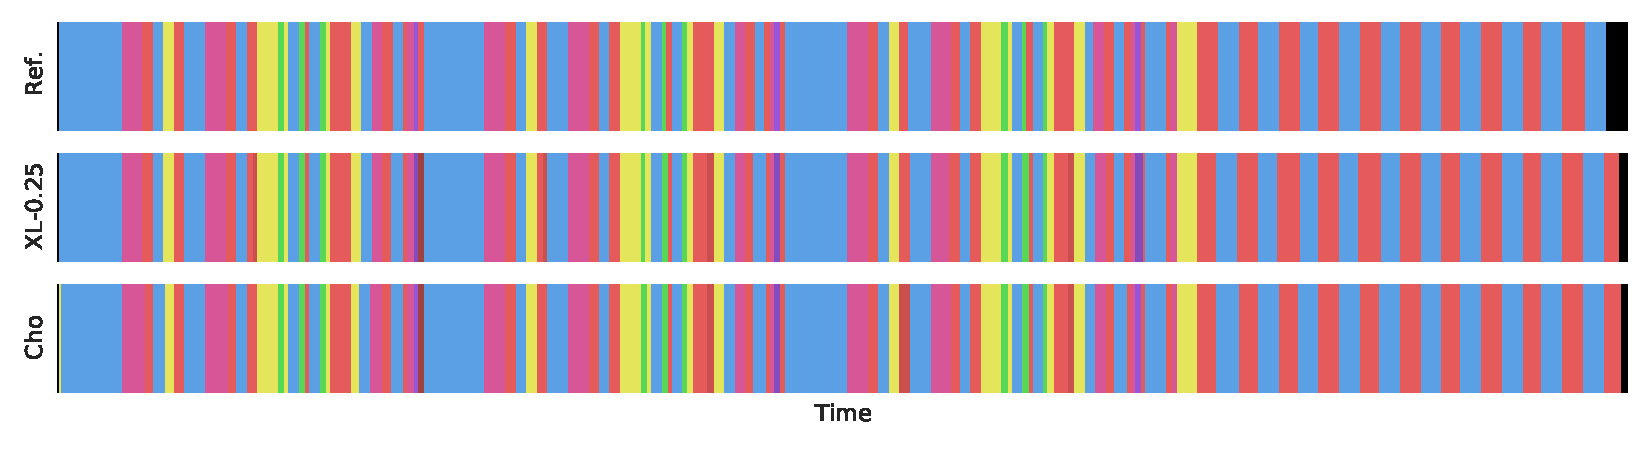
\includegraphics[width=\textwidth]{test_TRXHNQE149E2E0FFA2_annotations}
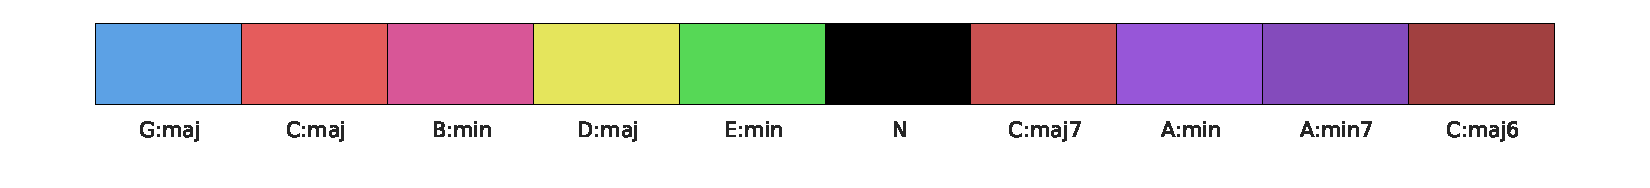
\includegraphics[width=\textwidth]{test_TRXHNQE149E2E0FFA2_legend}
\caption{Reference and estimated chord sequences for a track in quadrant I, where both algorithms agree with the reference.}
\label{fig:test_quadI}
\end{figure}


A track from quadrant I is given in Figure \ref{fig:test_quadI}.
As to be expected, the reference and both estimated chord sequences look quite similar.
The most notable discrepancy between the human-provided transcription and the two from the automatic methods is at the end of the sequence.
While the reference annotation claims that the transcription ends on a \texttt{G:maj}, both algorithms estimate the final chord as a \texttt{C:maj}.
This occurs because the song is in the key of G major, and thus the human chooses to end the song on the tonic chord.
However, the song ---``Against the Wind'' by Bob Seger--- is recorded with a fade-out, and the last audible part of the recording is in fact the \texttt{C:maj}, when playback volume is adjusted accordingly.
Therefore, this is an instance of the automatic systems being more precise than the human annotator.


\begin{figure}[t]
\centering
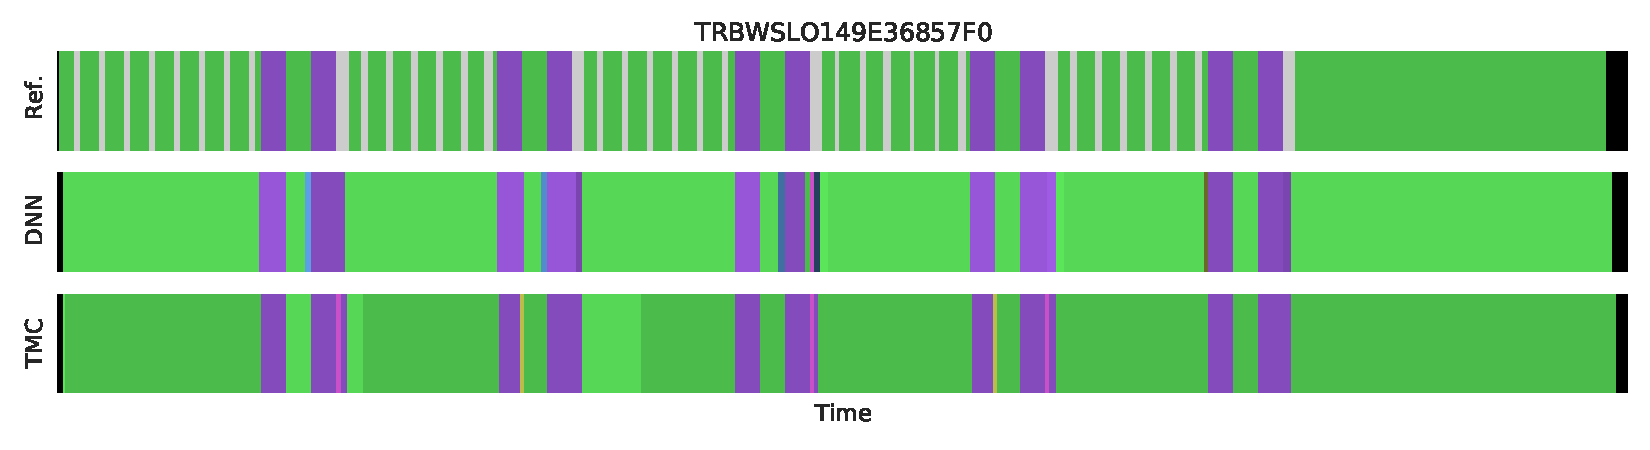
\includegraphics[width=\textwidth]{test_TRBWSLO149E36857F0_annotations}
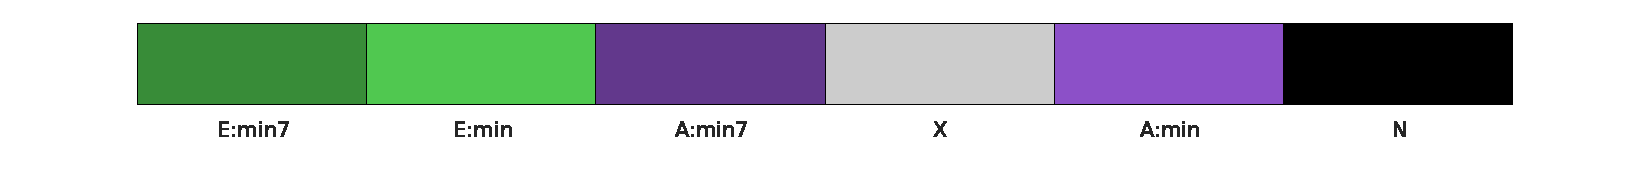
\includegraphics[width=\textwidth]{test_TRBWSLO149E36857F0_legend}
\caption{Reference and estimated chord sequences for a track in quadrant II, the condition where algorithms disagree sharply, but one agrees strongly with the reference.}
\label{fig:test_quadII}
\end{figure}

Next, a track from quadrant II ---``Smoking Gun'' by Robert Cray--- is considered in Figure \ref{fig:test_quadII}.
While the baseline system, TMC, agrees strongly with the reference that the predominant chord is an \texttt{E:min7}, the deep network, DNN, prefers \texttt{E:min}, and produces a poor ``tetrads'' score as a result.
This confusion is an understandable one, and highlights an interesting issue in automatic chord estimation evaluation.
Depending on the instance, it could be argued that some chords are not fundamentally different classes, and thus ``confusions'' in the traditional machine learning sense, but rather a subset of a more specified chord, e.g. \texttt{E:min7} $\supset$ \texttt{E:min}.
Traditional 1-of-k classifier schemes fail to encode this nuance, whereas a hierarchical representation would better capture this relationship.


\begin{figure}[t]
\centering
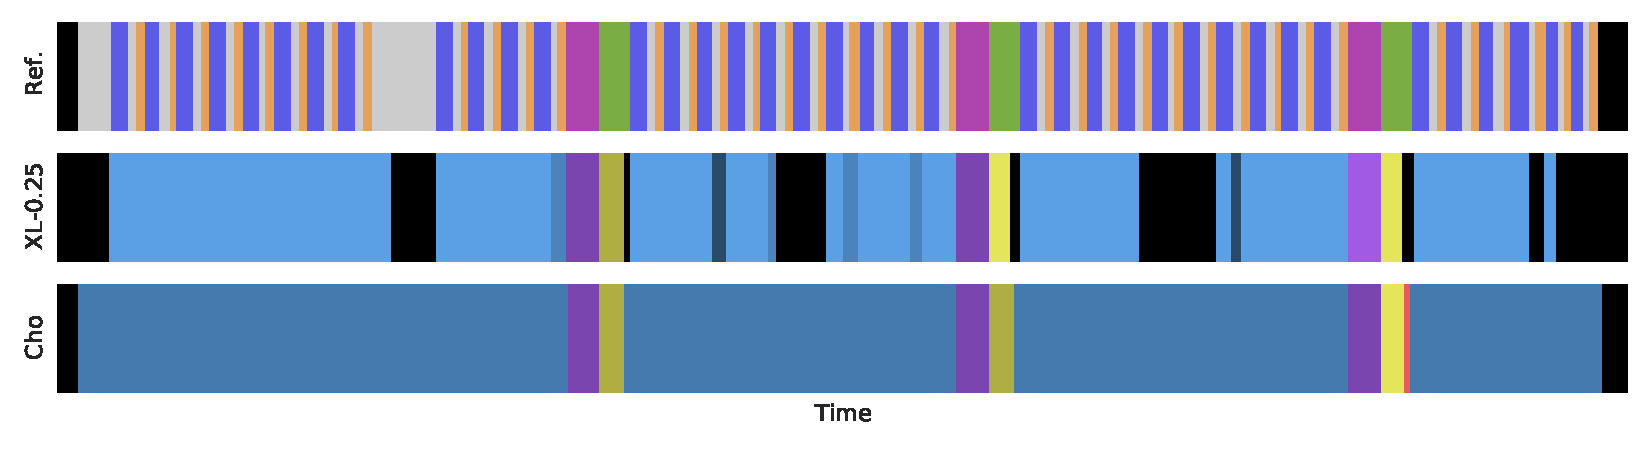
\includegraphics[width=\textwidth]{test_TRVVMUA149E3780587_annotations}
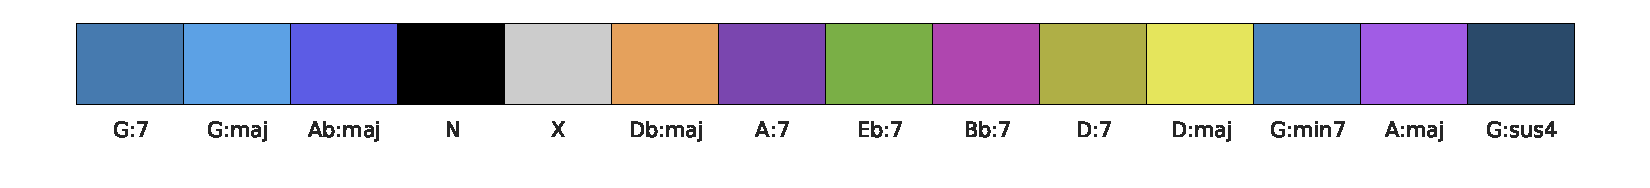
\includegraphics[width=\textwidth]{test_TRVVMUA149E3780587_legend}
\caption{Reference and estimated chord sequences for a track in quadrant III, the condition where neither algorithm agrees with the reference, nor each other.}
\label{fig:test_quadIII}
\end{figure}

The track drawn from quadrant III ---``Nowhere to Run'' by Martha Reeves and the Vandellas--- is shown in Figure \ref{fig:test_quad_III}, and especially interesting for three reasons.
First, most of the considerable disagreement between the reference and both estimated chord sequences can be explained by a tuning issue.
The automatic systems predict the tonic as \texttt{G}, while the human reference is based on \texttt{Ab}.
Matching a pure tone to this recording places the tonic around 400 Hz;
for reference to absolute pitch, the notes \texttt{G3} and \texttt{Ab3} correspond to roughly 391 Hz and 415 Hz, respectively.
Therefore, the human annotator and automatic systems disagree on how this non-standard tuning should be quantized.
Second, the two automatic systems again differ on whether to label the chord a \texttt{maj} or \texttt{7} chord; however, despite the tuning discrepancy, this time the reference annotation prefers the triad.
Lastly, there are three instrumental ``breaks'' in the piece where the backing band drops out to solo voice and drumset.
While this is indicated in the reference annotation in the first third of the song by an \texttt{X} chord label, the other two occurrences are not marked similarly.
The deep network model labels all three of these instances as no-chord, shown as black regions in the middle track.


\begin{figure}[t]
\centering
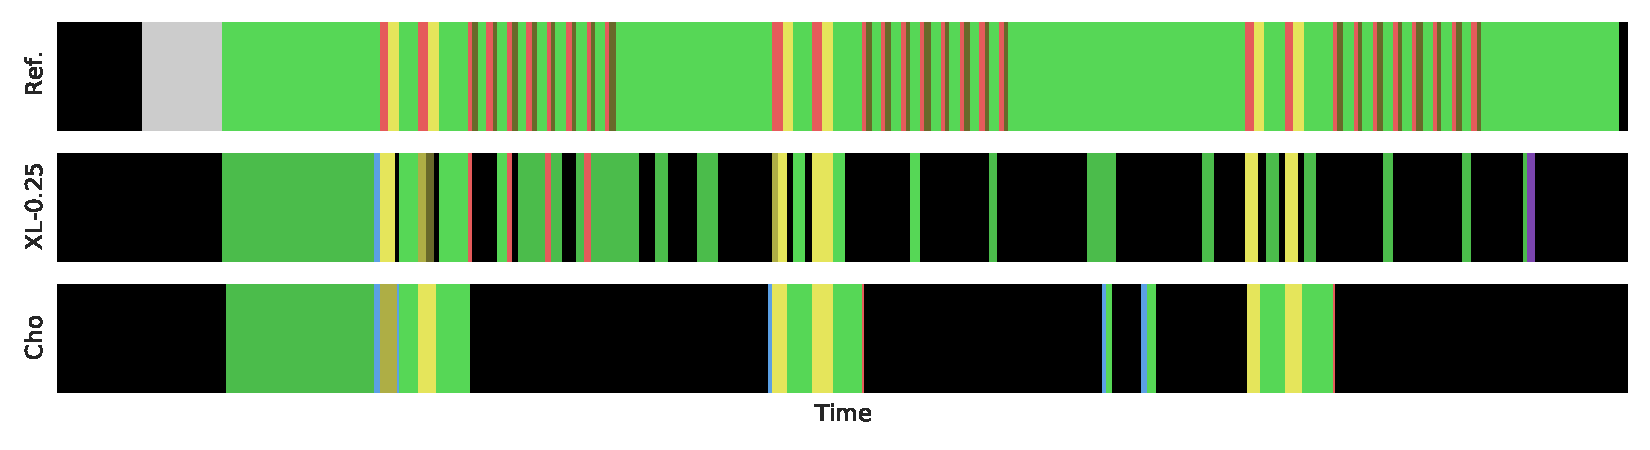
\includegraphics[width=\textwidth]{test_TRNFEEU149E38D3E18_annotations}
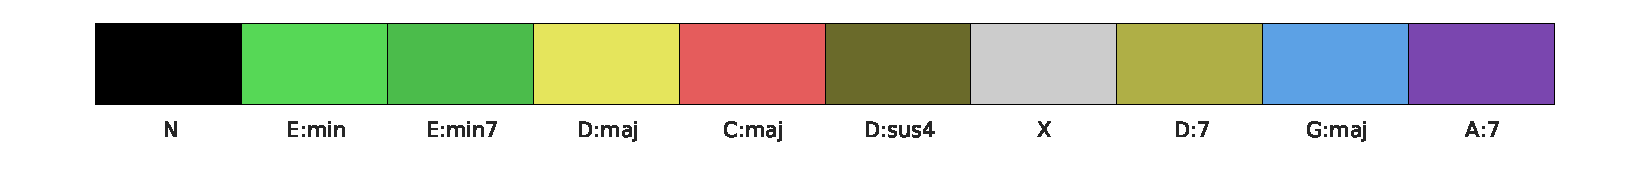
\includegraphics[width=\textwidth]{test_TRNFEEU149E38D3E18_legend}
\caption{Reference and estimated chord sequences for a track in quadrant IV, the condition where both algorithms agree with each other, but neither agrees with the reference.}
\label{fig:test_quadIV}
\end{figure}

As a final example from this analysis of two-part estimations, a track is considered from quadrant IV, shown in Figure \ref{fig:test_quadIV}, corresponding to ``Some Like It Hot'' by The Power Station.
Evidenced by the large regions of estimated no-chord, both automatic systems struggle on this particular track.
Listening through, there are likely two contributing factors.
One, the song is very percussive, and heavily compressed wideband noise probably disrupts the harmonic estimates made by the models.
Two, and perhaps more problematic, is that the song makes very little use of true pitch simultaneities, and much of the harmony in this song is implied.
Much of the song is sparsely populated from an instrumental perspective, and this less common musical arrangement results in erroneous estimations.
Importantly, both systems appear to fall victim to this deficiency, thus identifying an possible research area for future endeavors.



\subsection{Rock Corpus Analysis}
\label{subsec:qualitative_analysis}

Much can and has been said about the consistency, and thus quality, of the reference annotations used for development and evaluation of chord estimation systems.
The majority of human-provided chord annotations are often singular, either being performed by one person or as the result of a review process to resolve disagreements.
The idea of examining, rather than resolving, annotator disagreements is an interesting one, because there are two reasons why such discrepancies might occur.
The first is simply a matter of human error, resulting from typographical errors and other similar oversights.
The second, and far more interesting cause, is that there is indeed some room for interpretation in the musical content, leading to different acceptable annotations.
Most chord annotation curation efforts have made an explicit effort to resolve all discrepancies to a canonical transcription, however, and it is not possible to explore any such instances in the data used so far.



Fortunately, the \emph{Rock Corpus} dataset, first introduced in \cite{deClerqc2010}, is a set of 200 popular rock tracks with time-aligned chord and melody transcriptions performed by two expert musicians:
one, a pianist, and the other, a guitarist.
This insight into musical expertise adds an interesting dimension to the inquiry when attempting to understand alternate interpretations by the annotators.
This collection of chord transcriptions has seen little use in the ACE literature, as its initial release lacked timing data for the transcriptions, and the chord names are provided in a Roman Numeral syntax.
A subsequent release fixed the former issue, however, in addition to doubling the size of the collection.
The latter issue is more a matter of convenience, as key information is provided with the transcriptions and this format can be translated to absolute chord names, consistent with the syntax in Section \ref{subsec:chord_syntax}.
This dataset provides a previously uncapitalized opportunity to explore the behavior of ACE systems as a function of multiple reference transcriptions.


% What happens if the ground truth changes?

% Concurrent opinions are different from sequential opinions; this is known as ``anchoring'' and causes hysteresis in annotation.
% For example, ``Human A says X, human B doesn't disagree'' doesn't entail ``Human B says Y, human A disagrees''.

% What if either is ground truth? We can look at C(A, B) vs max(C(A, M), C(B, M)), over the rock corpus alone, to obtain many datapoints.
%

As an initial step, the two annotators, referred to here as DT and TdC, are each used as a reference and estimation perspective in order to quantify the agreement between them.
% Importantly, the chord vocabulary used by the RockCorpus transcriptions is a subset of all chords considered in this work, and no ef
The results, given in Table \ref{tab:rc_agreement}, indicate a high, but imperfect level of consistency between the two human perspectives.
Following earlier trends, this is also a function of the chord spelling complexity, whereby equivalence at the ``root'' is much higher than for ``tetrads''.
Additionally, it is worth noting the asymmetry in chord comparisons.
Thus, depending on the perspective used as the reference, a estimation may match better or worse with it.
Finally, it is curious that the ``MIREX'' score is not perfect, a measure that focuses on pitch composition rather than contextual spelling.
One would assume that the difficulty in naming a chord is more a function of the latter than the former, but this proves not to be the case.

\begin{table}[t]
\begin{center}
\scriptsize
\caption{Micro-recall scores for the two references against each other, each as the reference against a deep network, and either against the deep network.}
\label{tab:rc_agreement}

\begin{tabular}{lrrrrrrr}
\hline
         &   triads &   root &   mirex &   tetrads &   sevenths &   thirds &   majmin \\
\hline
DT vs TdC  &  0.8986 & 0.9329 &  0.9180  &   0.8355  &    0.8380  &   0.9042  &  0.9008 \\
TdC vs DT &   0.9117 & 0.9465 &  0.9168  &   0.8477  &    0.8537 &   0.9174 &    0.9176 \\
\hline
DT vs DNN  &   0.7051 & 0.7816 &  0.7180  &   0.5625   &   0.5653  &  0.7314  &  0.7084 \\
TdC vs DNN  & 0.7182 & 0.7939 & 0.7314  &   0.5786  &    0.5822 &   0.7444 &   0.7228 \\
\hline
(DT | TdC) vs DNN & 0.7306 & 0.8010 & 0.7431  &   0.5998  &    0.6032 &   0.7569  &  0.7348\\
\hline
\end{tabular}
\end{center}
\end{table}

Continuing, the deep network used in the previous analysis, XL-0.125, is again considered here.
Adopting a similar methodology as before, the estimations of the deep network are compared against both references seperately, as well as against the references together and taking the better match.
Overall performance is generaly worse than that observed over the holdout data in the previous investigation.
This is predominantly caused by a mismatch in the chord distributions between the datasets, as the RockCorpus only contains half the chords known to the automatic system.
Scores at the comparison of the ``root'' are much closer than that of the ``tetrads'' level, for example.
Comparing the algorithmic estimations against the intersection of the human references results in a small performance boost across all scores, indicating that the machine's ``errors'' are musically plausible, and might be validated by an additional perspective.


\begin{figure}[t]
\centering
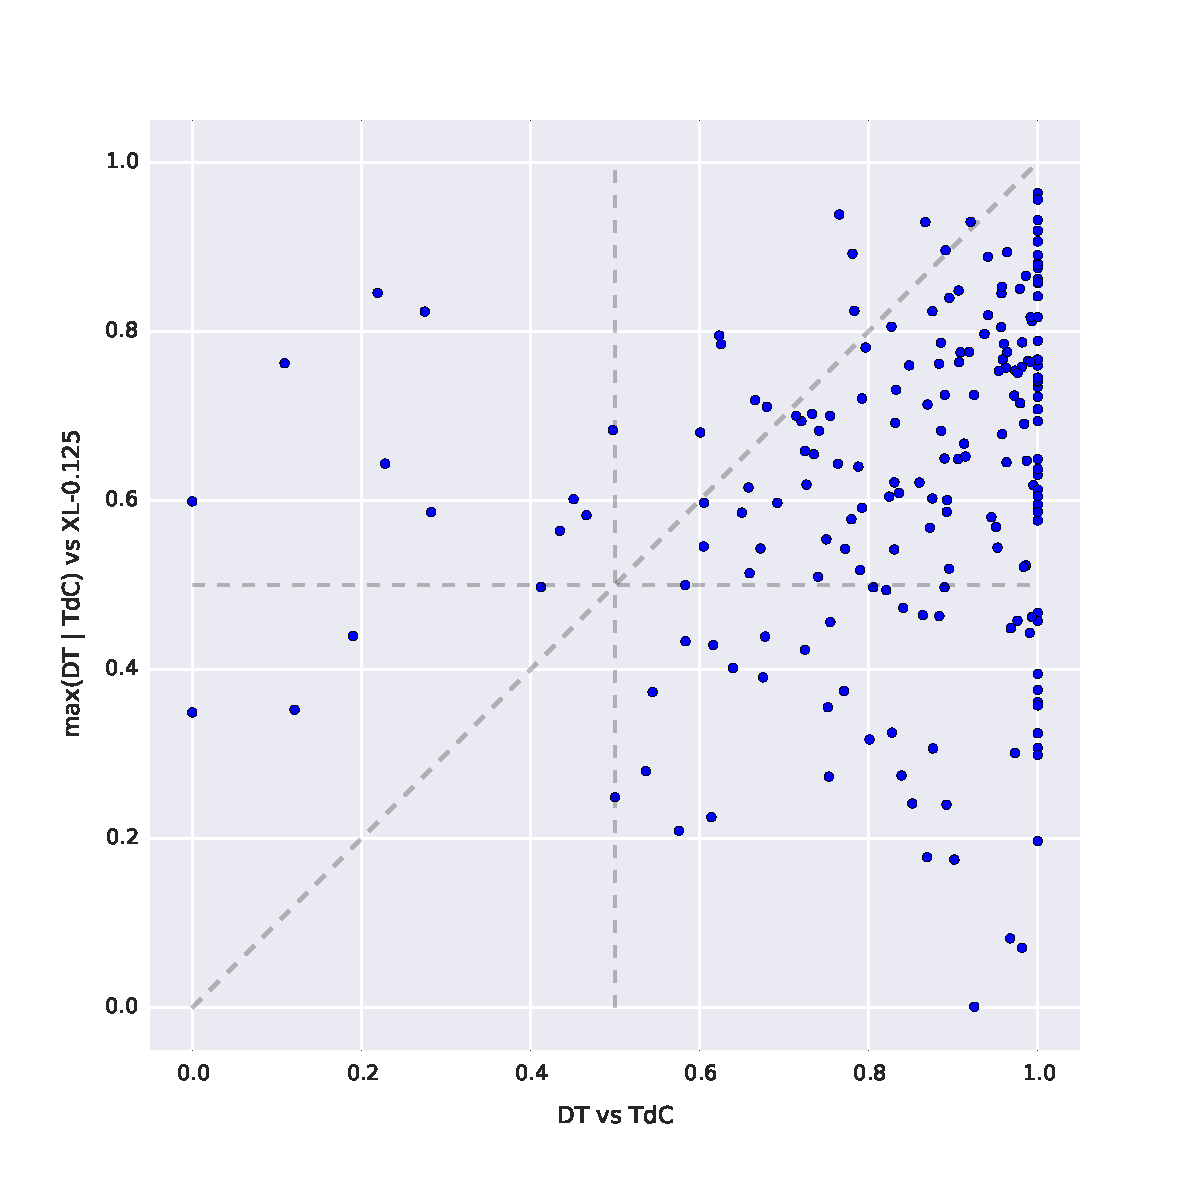
\includegraphics[width=\textwidth]{trackwise_rc_agreement}
\caption{Trackwise agreement between anotators versus the best match between either annotator and the best performing deep network.}
\label{fig:trackwise_rc_agreement}
\end{figure}

Keeping with previous methodology, annotator agreement is compared to the better match between the estimation and either reference on a trackwise basis; this is given in Figure \ref{fig:trackwise_rc_agreement} for the ``tetrads'' metric.
In contrast to Figure \ref{fig:trackwise_test_agreement}, the former is shown along the $x$-axis, and the latter along the $y$-axis.
This scatter plot can be understood similarly to before, with a few slight differences.
As before, Quadrant I contains tracks where all transcriptions agree estimation ($x > 0.5$, $y > 0.5$), and Quadrant III, where all transcriptions disagree ($x < 0.5$, $y < 0.5$).
Quadrant II now contains tracks where the \emph{annotators} disagree significantly ($x < 0.5$), but one annotator matches the reference well ($y > 0.5$), and Quadrant IV contains tracks where the annotators agree ($x > 0.5$), but the estimation disagrees with them both ($y < 0.5$).


\begin{figure}[t]
\centering
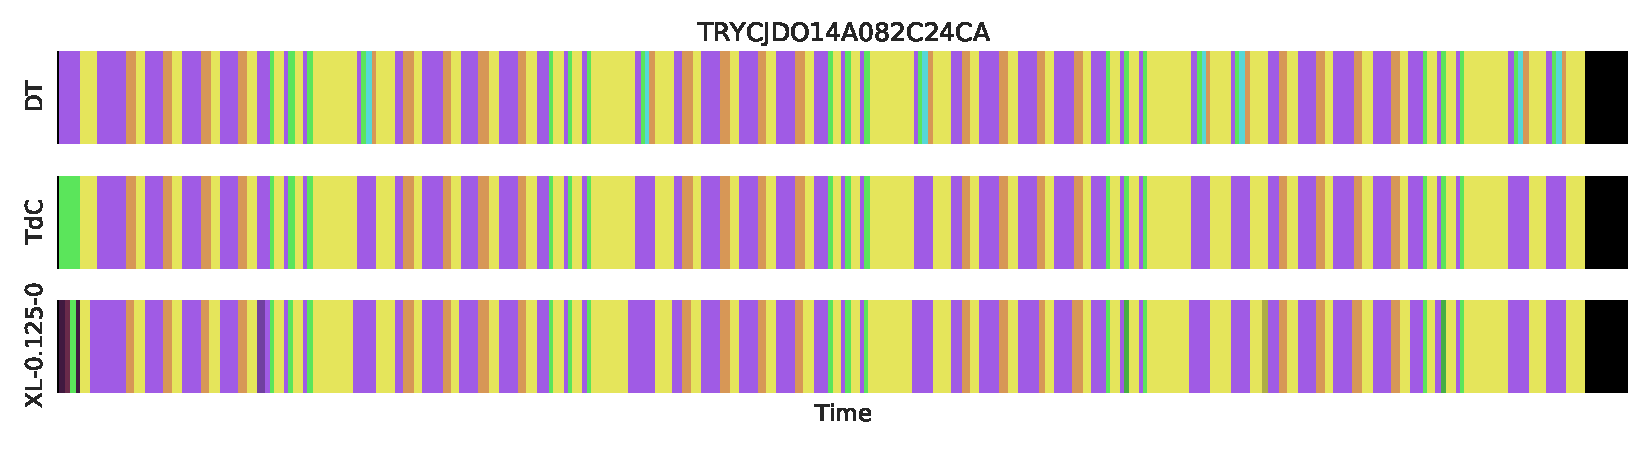
\includegraphics[width=\textwidth]{rc_TRYCJDO14A082C24CA_annotations}
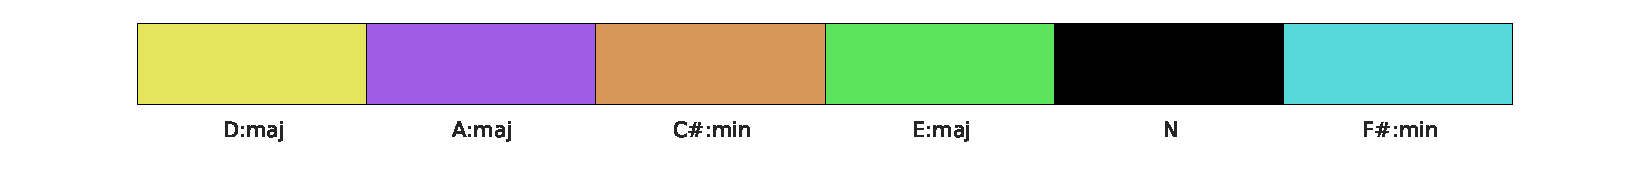
\includegraphics[width=\textwidth]{rc_TRYCJDO14A082C24CA_legend}
\caption{Reference and estimated chord sequences for a track in quadrant I, where the algorithm agrees with both annotators.}
\label{fig:rc_quadI}
\end{figure}

Figure \ref{fig:rc_quadI} shows the three-part transcription for ``The Weight'' by The Band, a track in Quandrant I.
Again, the three chord sequences score well against each other, and offer a high degree of visual similarity.
Notably though, the algorithmic estimation independently agrees more with the interpretation of TdC than DT.
For example, there are slight discrepancies in root movement at the end of the sequence, where DT expands the \texttt{A:maj} of TdC and DNN into \texttt{A:maj}-\texttt{F\#:min}-\texttt{C\#:min}, or relatively in Roman numeral form, I-vi-iii.
This motion occurs multiple times in the song, and each annotator's interpretation is internally consistent.

\begin{figure}[t]
\centering
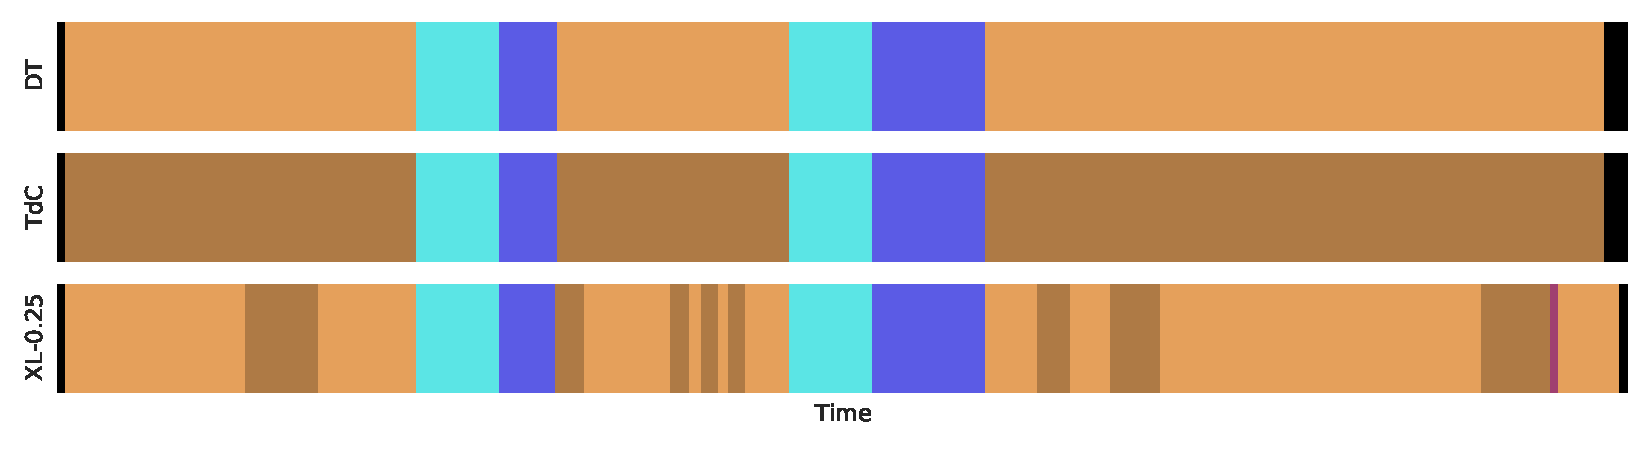
\includegraphics[width=\textwidth]{rc_TRJAZCU14A0814BC9D_annotations}
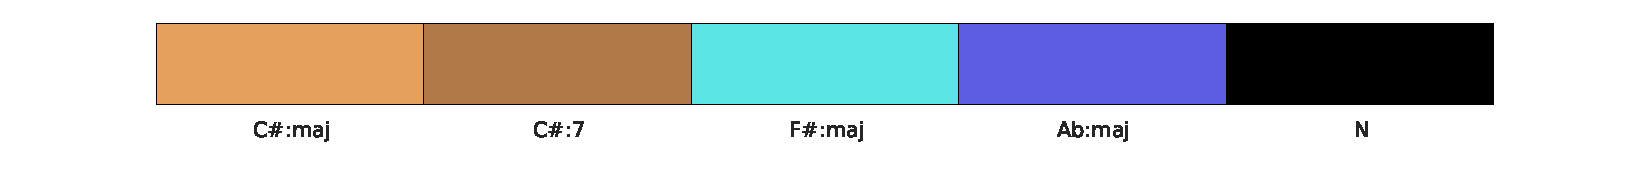
\includegraphics[width=\textwidth]{rc_TRJAZCU14A0814BC9D_legend}
\caption{Reference and estimated chord sequences for a track in quadrant II, the condition where the annotators disagree sharply, but one agrees strongly with the algorithm.}
\label{fig:rc_quadII}
\end{figure}

Being that the human annotators tend to agree more with each other than the two automatic systems previously considered, fewer tracks fall in the left half of the scatter plot in Figure \ref{fig:trackwise_rc_agreement} than Figure \ref{fig:trackwise_test_agreement}.
One of these from Quadrant II, ``All Apologies'' by Nirvana, is shown in Figure \ref{fig:rc_quadII}.
Here, the human annotators have disagreed on the harmonic spelling of the verse, with DT and TdC reporting \texttt{C\#:maj} and \texttt{C\#:7}, respectively.
On closer inspection, it would appear that both annotators are in some sense correct;
the majority of the verse is arguably \texttt{C\#:maj}, but a cello sustains the flat-$7^{th}$ of this key intermittently.
% 27 seconds in
These regions that this occurs are clearly captured in the DNN annotation, corresponding to its \texttt{C\#:7} predictions.
This proves to be an interesting discrepancy, because one annotator (DT) is using long-term structural information about the song to apply a single chord to the entire verse.

\begin{figure}[t]
\centering
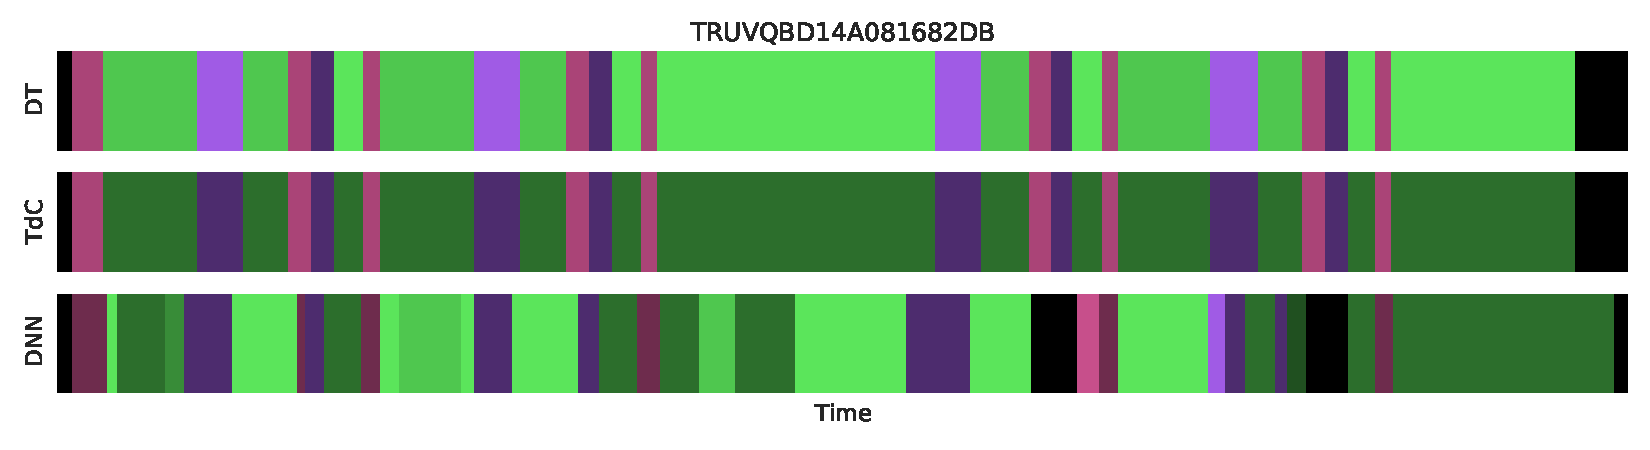
\includegraphics[width=\textwidth]{rc_TRUVQBD14A081682DB_annotations}
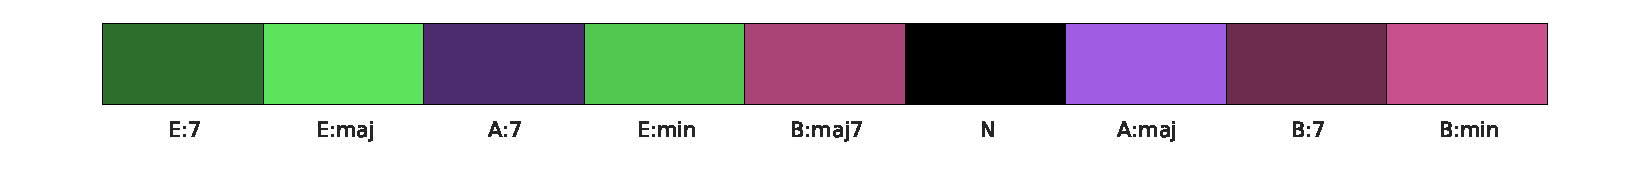
\includegraphics[width=\textwidth]{rc_TRUVQBD14A081682DB_legend}
\caption{Reference and estimated chord sequences for a track in quadrant III, the condition where neither annotator agrees with the algorithm, nor each other.}
\label{fig:rc_quadIII}
\end{figure}

Another of these select few, this time from Quadrant III, is ``Papa's Got a Brand New Bag'' by James Brown, shown in Figure \ref{fig:rc_quadIII}.
In this instance, all perspectives involved disagree substantially, not only at the level of sevenths but also the quality of the third.
Exploring why this might be the case, one finds the song consists of unison riffs and syncopated rhythms with liberal use of rests.
In the absence of sustained simultaneities, most of the harmony in the song is implied, creating even more room for subjectivity on behalf of the annotators.
The automatic system, alternatively, flips back and forth between the various perspectives of the two reference annotations.
Again, the system tends to be rather literal in its interpretation of solo vocal phrases, and labels such regions ``no-chord'' in the middle of the song.


\begin{figure}[t]
\centering
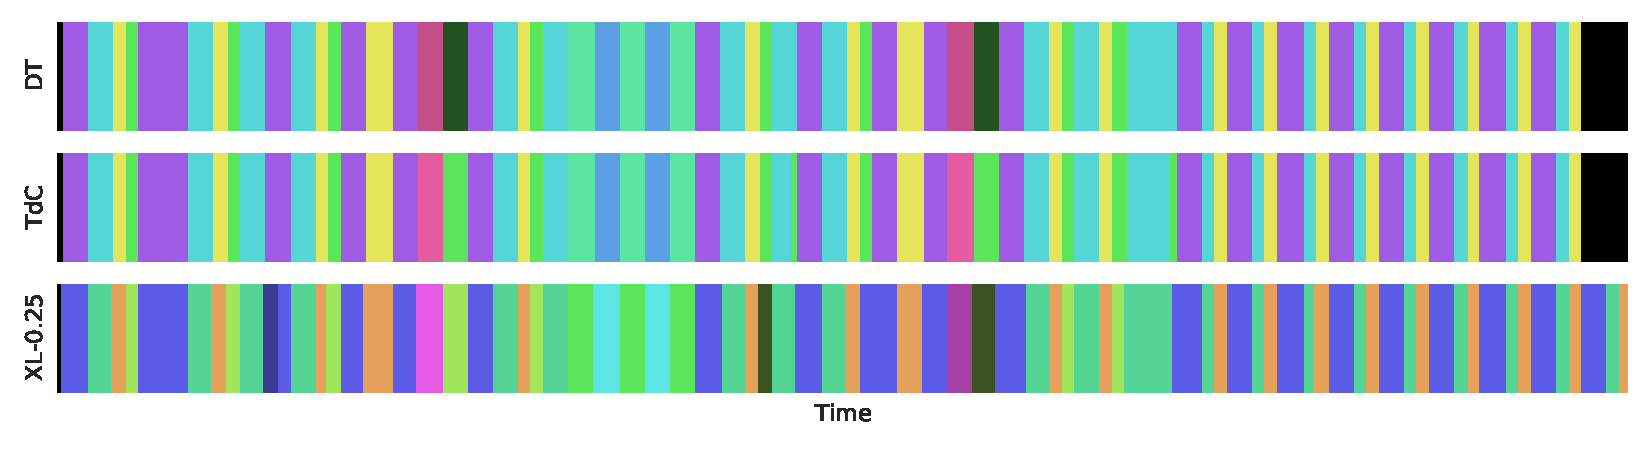
\includegraphics[width=\textwidth]{rc_TRXVZFX14A0816D7D2_annotations}
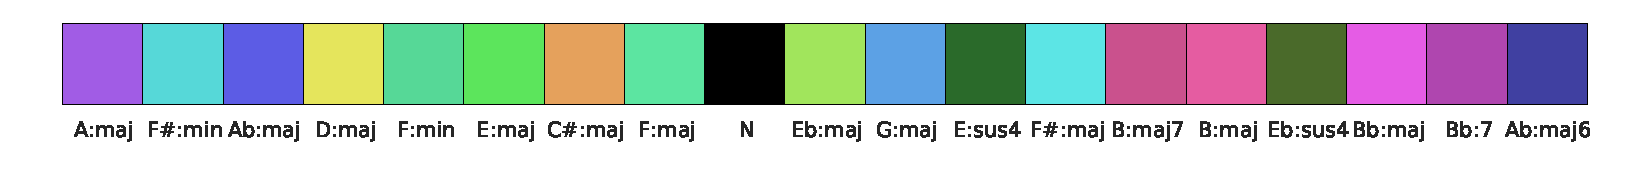
\includegraphics[width=\textwidth]{rc_TRXVZFX14A0816D7D2_legend}
\caption{Reference and estimated chord sequences for a track in Quadrant IV, the condition where both annotators agree with each other, but neither agrees with the algorithm.}
\label{fig:rc_quadIV}
\end{figure}

Finally, a track from Quadrant IV ---``Every Breath You Take'' by The Police--- is given in Figure \ref{fig:rc_quadIV}.
Similar to the track considered from the same region before, the estimation is consistently a half-step flat from the references.
This pattern is indicative of a similar tuning discrepancy as before, and tuning a pure sinusoid to the track finds the tonic at approximately 426Hz, putting the song just over a quartertone flat.
Though functionally equivalent to the previous example of tuning being an issue, this instance is interesting because two annotators independently arrived at the same decision.
% Why would they both make the same mistake? Maybe it's not a mistake!
One reason this might have occurred is that, as a rock song, it makes far more sense to play in \texttt{A:maj} on guitar than \texttt{Ab:maj}.
The chord shapes involved are much easier to form in \texttt{A:maj}, and therefore more likely.
Additionally, a guitarist would probably need to change tunings to play the \texttt{Eb:maj} in the right voicing.
Taken together, it is noteworthy that such extrinsic knowledge can, and perhaps should, play a role in the process of automatic chord estimation.



\subsection{Conclusions \& Future Work}
\label{subsec:conclusions}

% Quantitative observations
Based on conventional methodology, the proposed deep learning approach leads to results on par with the state of the art, just eclipsing the baselie in the various metrics considered.
Though fully convolutional models can be complex enough to overfit the dataset, a small amount of dropout during training helps reduce this overfitting, while leading to slightly better generalization.
Dropout also raises quality-wise recall in minority classes significantly.
Given the significant imbalance of chord classes in the dataset, however, this is a very unstable measure of system performance.
Small shifts in the macro-recall of a majority class can result in large performance swings, and vice versa.
Thus, the criteria for what makes for a ``good'' system may be motivated by use case, to determine which of these metrics correspond to the desired behavior.

Additionally, the suite of chord comparison functions demonstrate that most errors between reference and estimation are hierarchical, and increase with specificity of the chord, e.g. from root to triads to tetrads.
One-of-K classifiers struggle to encode these relationships between certain chords, e.g. \texttt{A:maj} and \texttt{A:maj7}.
By analogy, this is like building a classifer that discriminates between, among other classes, animals and cats, respectively; all cats are animals, but not all animals are cats.
This is problematic in a flat classifier, because it is attempting to linearly separate a pocket of density contained within another.
To address this issue, a structured output and loss function would be better suited to model these relationships.
Directly encoding the knowledge that \texttt{maj7} chords are a subset of \texttt{maj}, will make it easier for a machine to learn these boundaries.
One such hierarchy for the chords considered in this work is given in Figure \ref{fig:chord_hierarchy}.
Here, the degree of specificity increases as the decision tree is traversed to a leaf node, and could be achieved with more structured output, such as a hierarchical softmax or conditional estimator.


\begin{figure}[t]
\centering
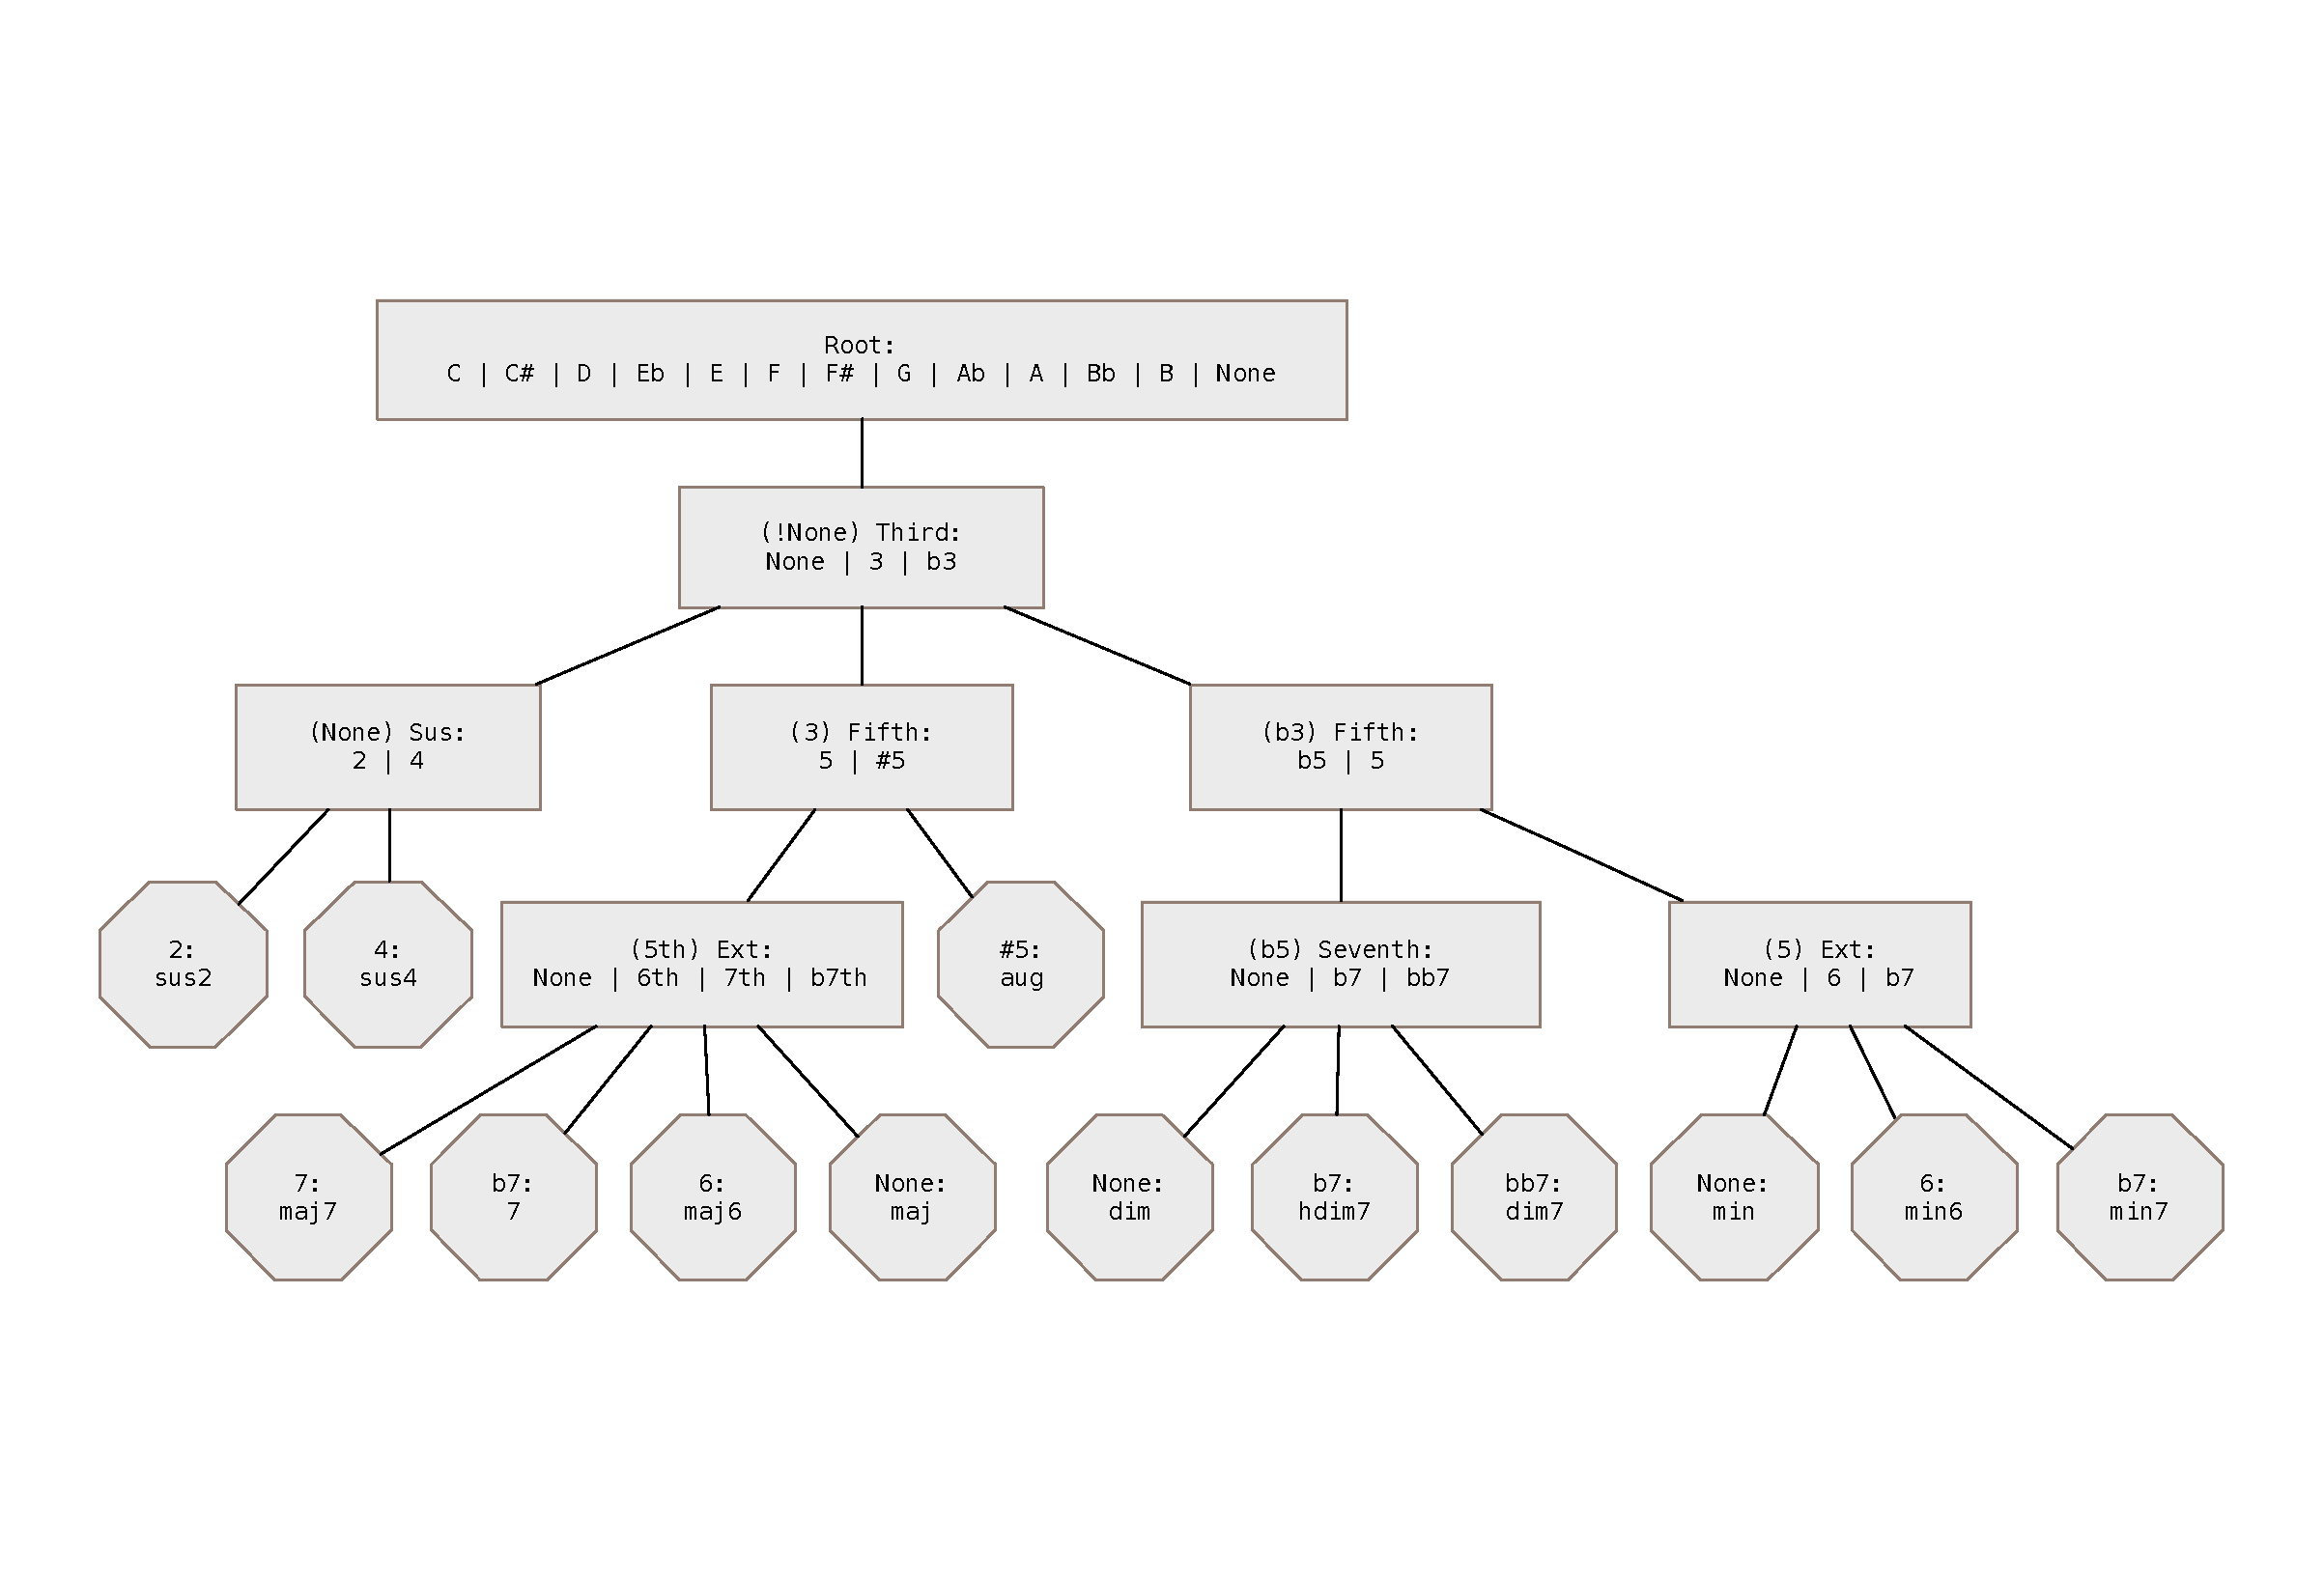
\includegraphics[width=\textwidth]{chord_hierarchy}
\caption{A possible chord hierarchy for structured prediciton of classes. Decisions blocks are rectangular, with the result of the previous node shown in parentheses, the semantic meaning of the node is given before a colon, and the set of valid responses is pipe-separated. Stopping conditions are given as octagons.}
\label{fig:chord_hierarcy}
\end{figure}


% On having mutliple estimators
In comparing the estimations of the two computational systems, deeper insight is gained into the ground truth data used for development, and the kinds of behavior, both the good and bad, that such approaches are prone to exhibit.
First, it is observed that they make rather different predictions and their responses could be combined, motivating the exploration of ensemble methods.
Looking at performance at the track-level, alternatively, helps identify problematic or noisy data in a collection.
This is similar in spirit to a growing body of work in MIR \cite{Holzapfel}, but it also provides some unique insight into the ACE task itself.
Computational systems tend to be precise in ways humans are not, such as continuing to predict chords during a fade-out, or reporting ``no-chord'' during a musical break.
The issue of hierarchical class relationships manifests in both models, but instances of algorithm disagreement point to music content that falls near a boundary between classes.
Such knowledge could be used to single out and review the reference chord annotation more closely.
These systems can also be sensitive to inexact tuning, and half-step deviations can be a large source of error.
Additionally, implied harmony or stacatto patterns can be especially problematic, resulting in an over-estimation of the ``no-chords'' class.


% On having multiple annotators
Conversely, leveraging multiple annotations for a given track provides a deeper understanding of the errors a computational system might make.
As seen here, the assessment of a system will change depending on which interpretation is taken as a reference, and a computational system may agree with another human's perspective, consistent with the work of McVicar \cite{McVicar}.
Most imporant is the recognition that human annotators do not agree all the time, and that describing some music content in the language of chords is inherently subjective.
In such cases, there is no ``ground truth'' to speak of, and multiple chord labels may be acceptable.
This is a critcal observation, and one that cuts strongly against the long-standing methodology of curating ground truth references in ACE.
Stated previously, the sole purpose of an objective measure is that it serves as a reasonable proxy for subjective experience.
If the goal of ACE is to produce a chord annotation on par with that of a qualified human ---a musical Turing test of sorts--- then the reference annotation at hand may be only one of many valid perspectives.
As a result, evaluating against a singular perspective is leading to results that may be inconsistent with subjective experience.

Instead, embracing multiple perspecives, rather than attempting to resolve them into a canonical target, would allow for more stable evaluation of computational models.
One such way this could be achived is by obtaining multiple chord annotations and creating a time-aligned bag of words reference.
For example, knowing that 97 of 100 annotators labeled a chord as \texttt{A:7} is very different from the scenario that 52 did, while the other 48 reported \texttt{A:maj}.
Curating a dataset with so many perspectives is unlikely to happen, but perhaps multiple computational systems could be used to find boundary chords that \emph{do} warrant multiple perspectives.
Ultimately, this study demonstrates that future chord datasets should strive to capture the degree of subjectivity in an annotation, thus enabling objective measures better correspond with subjective experience.


\section{Summary}
\label{sec:summary}

In this chapter, the application of deep learning to ACE has been thoroughly explored.
By standard evaluation practices, competitive performance is demonstrated on both a major-minor and large-vocabularly formulation of the task.
Importantly, much effort is invested in understanding both the behavior of the computational systems discussed, as well as the reference data used to evaluate performace.
Perhaps the most important finding is that the current state of the art may have truly hit a glass ceiling, due to the conventional practice of building and testing against ``ground truth'' datasets for an inherently subjective task.
This challenge is further compounded by approaches to prediction and evaluation, which attempt to perform flat classification of a hierarchically structured chord taxonomy.
Thus, while there is almost certainly room for improvement, the exploration here indicates that the vast majority of error in modern chord recognition systems is a result of invalid assumptions baked into the very task.

Notably, four issues with current chord estimation methodology have been identified in this work.
One, it seems necessary that computational models embrace structured outputs; one-of-K class encoding schemes introuduce unnecessary complexity between what are naturally hierarchical relationships.
Two, the community fundamentally needs to better distinguish between the two tasks at hand, being chord recognition ---I am playing this literal chord on guitar--- and chord transcription ---finding the best chord label to describe this harmonically homogenous region of music--- and how this is articulated to reference annotation authors.
Three, chord transcription requires more explicit segmentation, rather than letting such boundaries between regions of harmonic stability result implicitly from post-filtering algorithms.
Lastly, the often subjective nature of chord labeling needs to be acknowledged in the process of curating reference data, and the human labeling task should average or combine multiple perspectives rather than attempt to yield a canonical ``expert'' reference.
